\documentclass[10pt, UKenglish]{beamer}
\usepackage{babel}
\usepackage[utf8]{inputenc}  
\usepackage{geometry}
\usepackage[customcolors]{hf-tikz}
\usepackage[T1]{fontenc}   
\usepackage{tcolorbox}
\usepackage{siunitx}
\usepackage{hyperref}
\usepackage{bookmark}
\usepackage{marvosym}
\usepackage{tikz}
\usepackage{tikz-qtree}
\usepackage{cancel}
\usepackage{todonotes}
\useoutertheme[subsection=false]{smoothbars}
\DeclareSIUnit[number-unit-product = {}]{\inchQ}{\textquotedbl}
\usepackage{amsmath,bm}
\DeclareSIUnit[number-unit-product = {\thinspace}]{\inch}{in}
\usetheme[menuwidth={0.3\paperwidth}]{erlangen}
\usepackage{multicol}
\usepackage{charter}
\setbeamercovered{transparent=20}
\setbeamertemplate{navigation symbols}{}
\sisetup{separate-uncertainty = true}
\usepackage[version=4]{mhchem}
\usepackage{tikz}
\usepackage{hepnames}
\usepackage{soul}
\usepackage{color}
\usepackage{thesis_defs}
\usepackage{subcaption}
\captionsetup[subfigure]{labelformat=empty}
\usepackage{xcolor}


\usepackage[backend=biber]{biblatex}
\bibliography{bibliography.bib}

\graphicspath{%
  {./feynman_diagrams/}%
  {./figures_theory/}%
  {./figures_simple/}%
  {./figures_misc/}%
  {./app1/}%
  {./app2/}%
  {./app3/}%
}


\definecolor{color1}{RGB}{33,217,217}
\definecolor{color2}{RGB}{7,61,111}

\newcommand{\lr}{\mathcal{lr}}


\newcounter{totavalue}
\newcounter{parvalue}

\def\aux{1}
\def\radius{9pt}
\def\step{4pt}
\usepackage[absolute,overlay]{textpos}


\newcommand\circcounter{%
\ifnum\inserttotalframenumber<2\relax
\else
  \setcounter{totavalue}{\inserttotalframenumber}
  \setcounter{parvalue}{\insertframenumber}
  \ifnum\inserttotalframenumber>45\relax
    \renewcommand\step{0pt}
  \fi%
  \pgfmathsetmacro{\aux}{360/32}
  \begin{tikzpicture}[remember picture,overlay, rotate=90+\aux]
  \foreach \i in {0,1,...,32}
    \fill[logo_blue] 
      (0,0) -- (-\i*\aux:\radius) arc  (-\i*\aux:-(\i+1)*\aux+\step:\radius) -- cycle;
  \foreach \i in {1,...,\insertframenumber}
    \fill[logo_grey] 
      (0,0) -- (-\i*\aux:\radius) arc  (-\i*\aux:-(\i+1)*\aux+\step:\radius) -- cycle;
  \fill[white] circle (\radius/1.3);
  \node at (0,0) {\small\insertframenumber}; 
  \end{tikzpicture}%
\fi%
}


\usepackage{eso-pic,picture}



\begin{document} 

\title[Bachelorvortrag]{Hyperparameter Optimisation of an Adversarial Neural Network in the \tW channel at \SI{13}{\tera \electronvolt} with ATLAS}
\subtitle{4th April 2019}
\author{Christian Kirfel}
%\institute{Universtität Bonn}
        



\begin{frame}[plain]
\vspace{0.0cm}
  \titlepage
      \AddToShipoutPictureFG*{%
    \AtPageUpperLeft{%
      \put(8.7cm,-9.6cm){

\includegraphics[scale=0.03]{original_logo.jpg}
\makebox(0,0)[lt]{}%
      }%
    }%
  }%
    \AddToShipoutPictureFG*{%
    \AtPageUpperLeft{%
      \put(0.0cm,-9.6cm){
%
\includegraphics[scale=0.17]{atlas_gay.png}

\includegraphics[scale=0.17]{ATLAS-Logo-Ref-RGB-H_0.jpg}
\makebox(0,0)[lt]{}%
      }%
    }%
  }%
\end{frame}
\addtobeamertemplate{navigation symbols}{\vspace*{0.8cm}\hfill\circcounter\hspace*{0.7cm}}

\section{Outline}

\begin{frame}{Outline}
\begin{itemize}%[<+-| alert@+>]
    \item The Standard Model of particle physics
    \vspace{0.5cm}
    \item Introducing the \tW channel
    \vspace{0.5cm}
    \item The LHC and the ATLAS detector
    \vspace{0.5cm}
    \item Neural networks in particle physics
    \vspace{0.5cm}
    \item Results for different approaches of adversarial neural networks
\end{itemize}
\end{frame}


\section{Setting the scene}

\begin{frame}{The standard model of particle physics}
\begin{columns}
\begin{column}{0.6\textwidth}
\begin{figure}
    \centering
    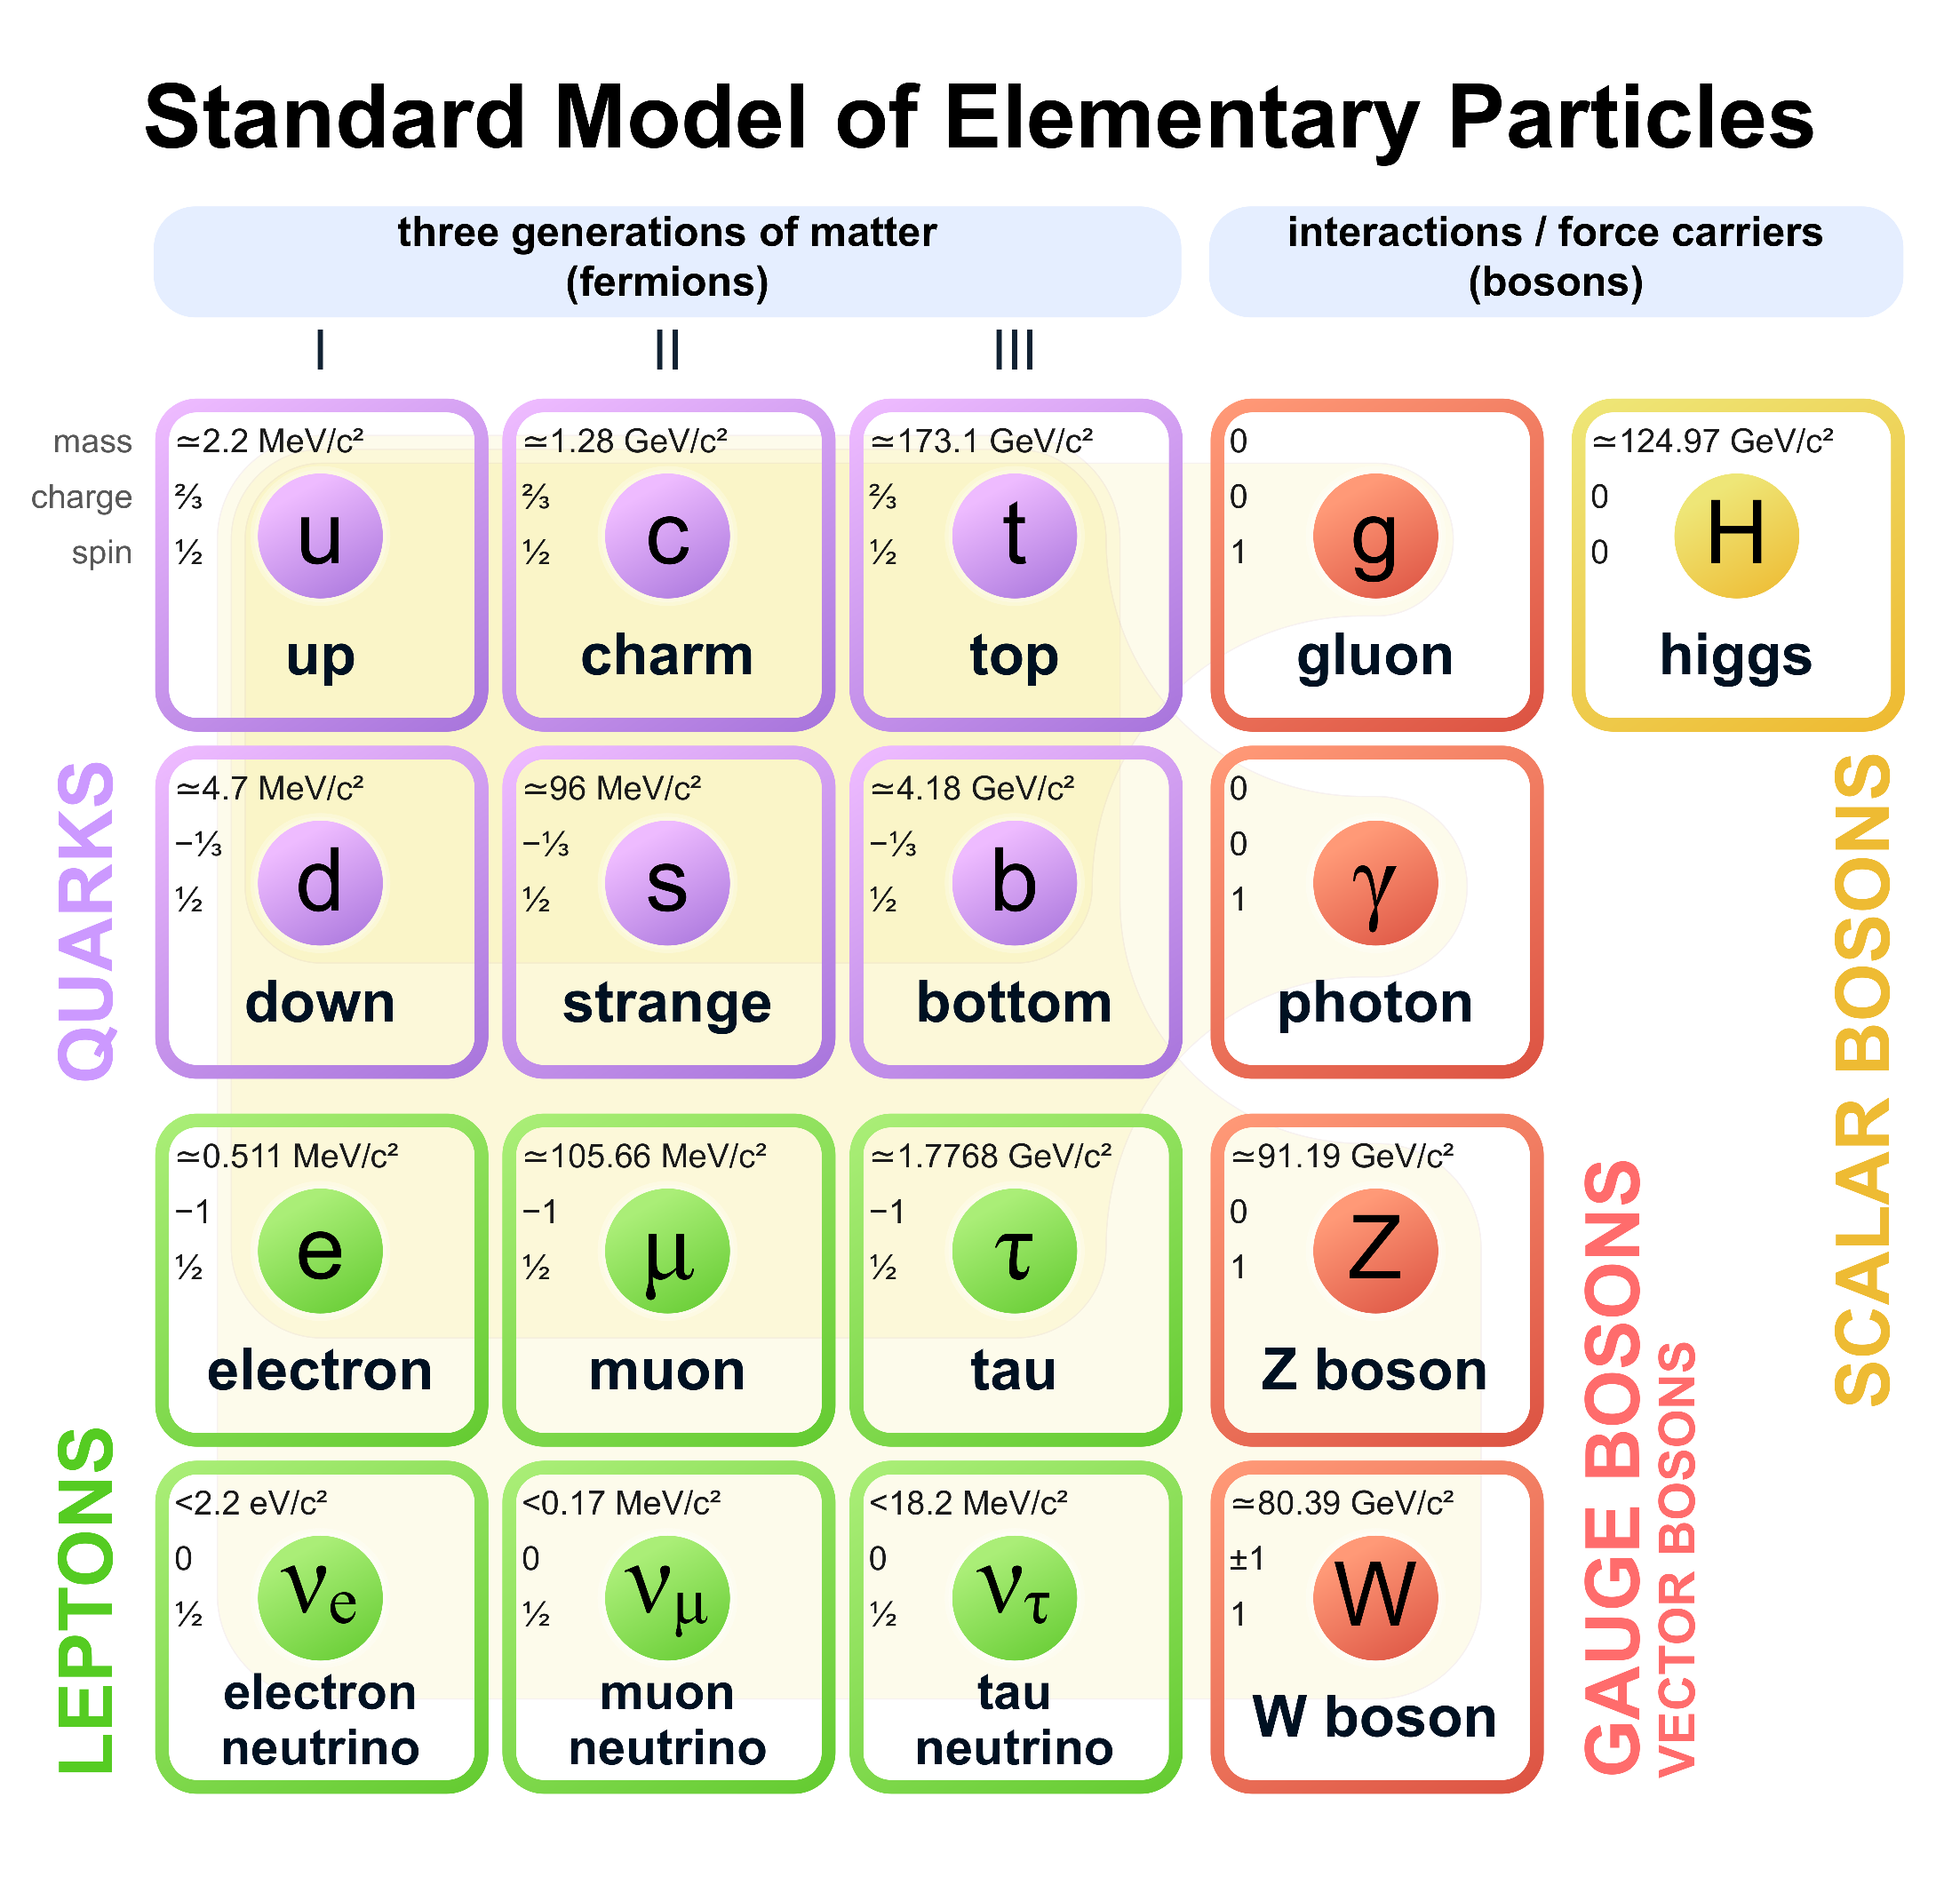
\includegraphics[scale=0.17]{Standard_Model_of_Elementary_Particles.eps}
\end{figure}
\end{column}
\pause
\begin{column}{0.4\textwidth}
\begin{block}{The top-quark}
        \begin{itemize}
            \item $ m \sim \SI{173}{\GeVovercsq}$
            \vspace{0.2cm}
            \item $\tau \sim \SI{5e-25}{\second}$
            \vspace{0.2cm}
            \item Lifetime < typical hadronisation time 
            \vspace{0.2cm}
            \item Decay into a \Pbottom-quark and a \PW-boson
        \end{itemize}
\end{block}
\end{column}
\end{columns}

\end{frame}

\begin{frame}{Top production}
    \begin{columns}
        \begin{column}{0.5\textwidth}
            \vspace{-0.4cm}
        \begin{block}{\tW single top production}
        \end{block}
			\begin{figure}
	            \centering
	            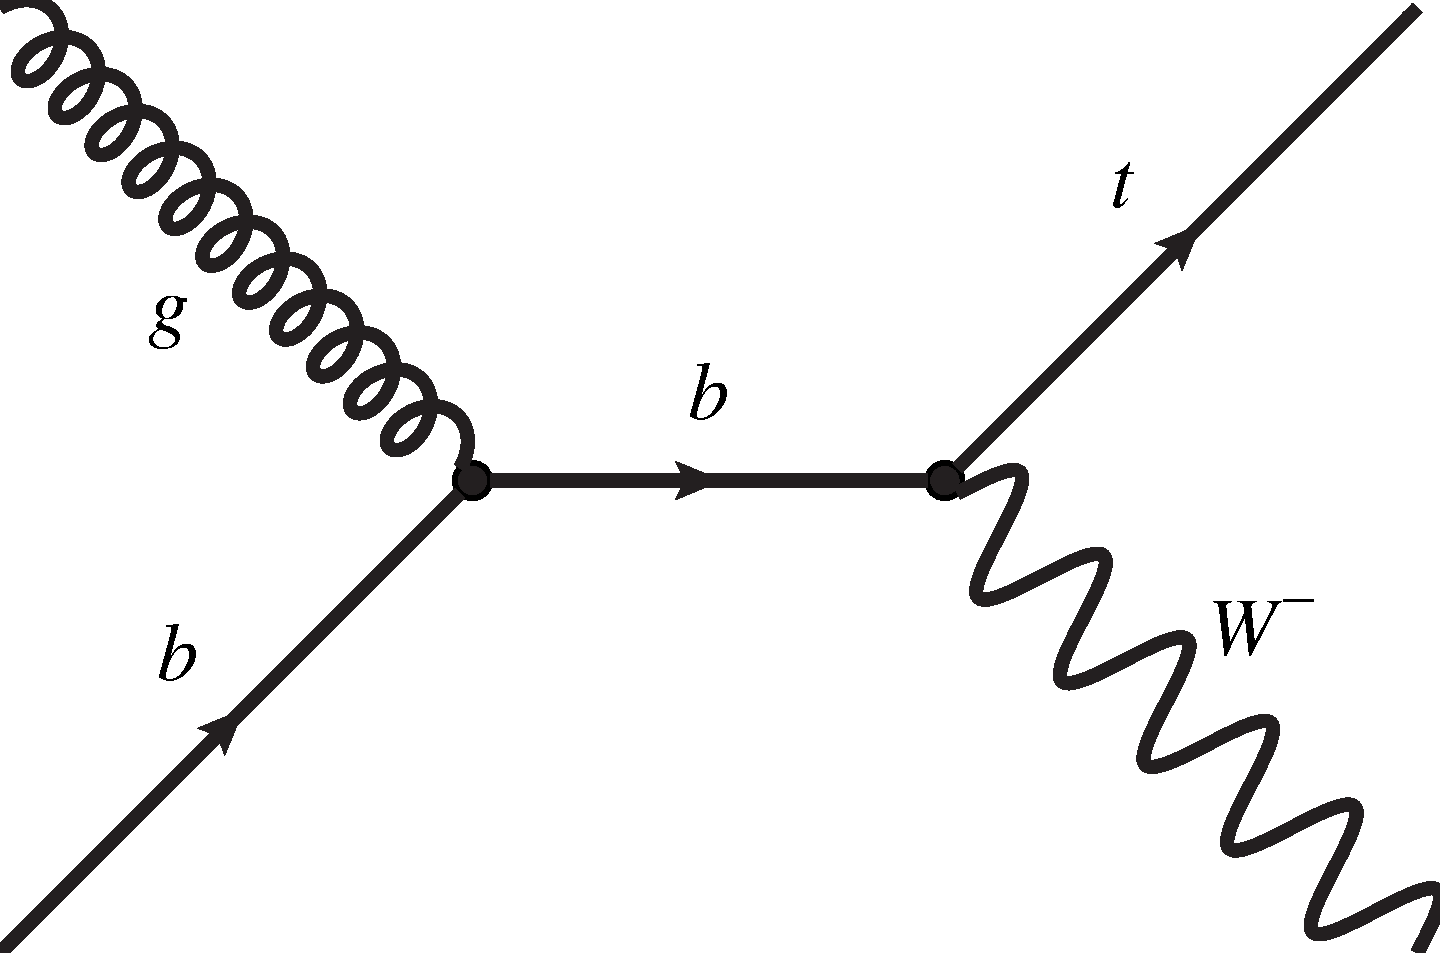
\includegraphics[width=0.8\textwidth]{tW_channel}
	        \end{figure}
	        \begin{itemize}
	        \item Via weak interaction
	        \item Relatively small cross-section
	        \end{itemize}
        \end{column}
        \begin{column}{0.5\textwidth}
        \begin{block}{\ttbar pair production}
        \end{block}
        \begin{figure}
            \centering
            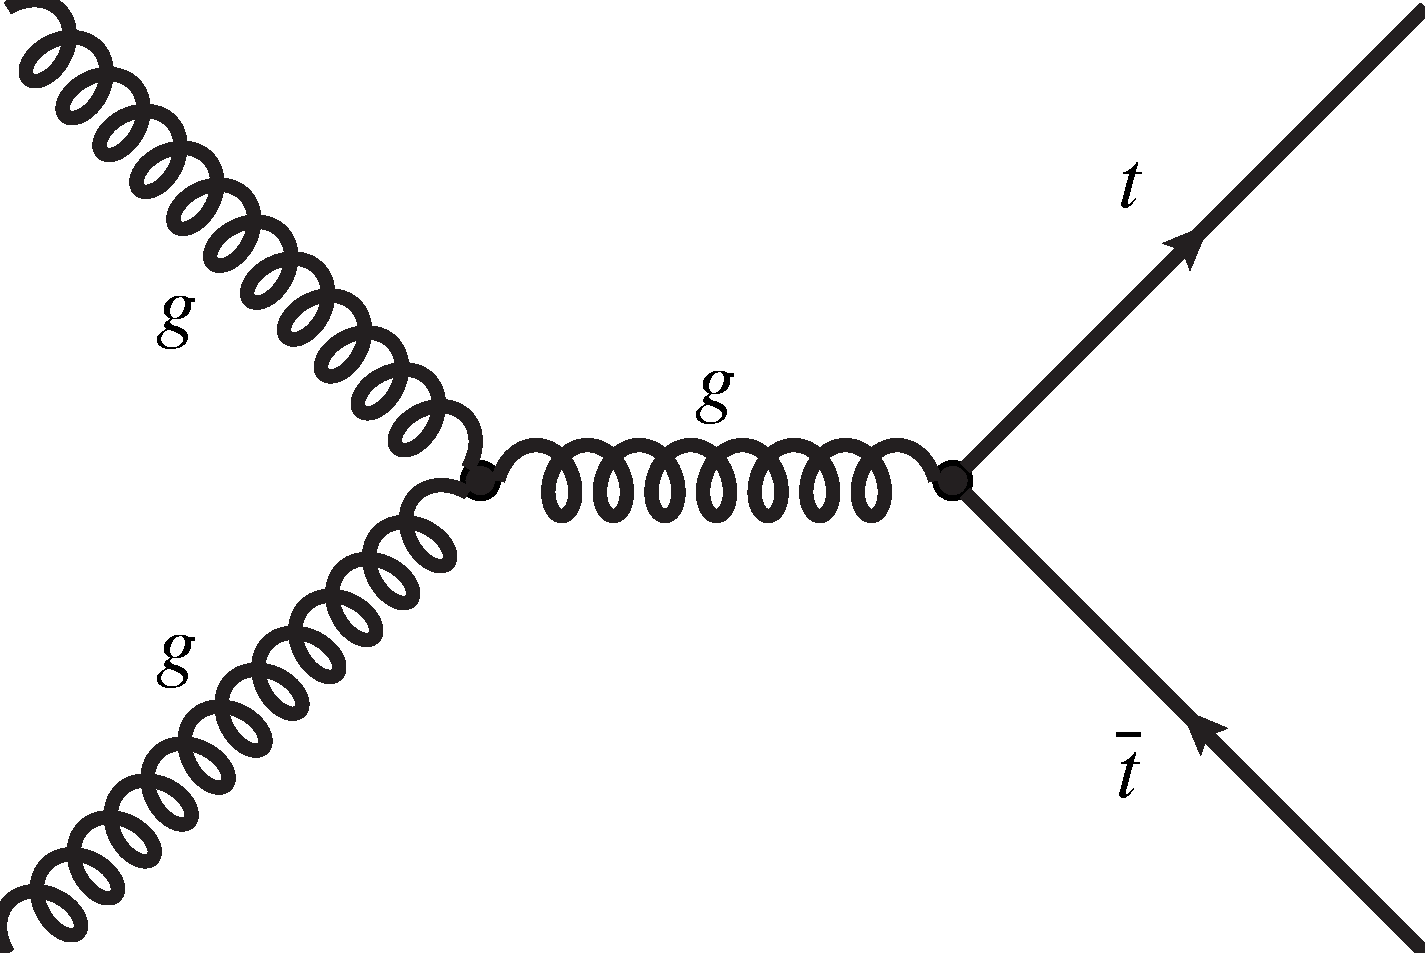
\includegraphics[width=0.8\textwidth]{ttbar_ttbar_1-BW}
        \end{figure}
        \begin{itemize}
        	\item Via strong interaction
        	\item More than 10 times the cross-section
        \end{itemize}
        \end{column}
    \end{columns}
\end{frame}

\begin{frame}{The Large Hadron Collider - LHC}
\begin{columns}
\begin{column}{0.7\textwidth}
\begin{figure}
        \centering
        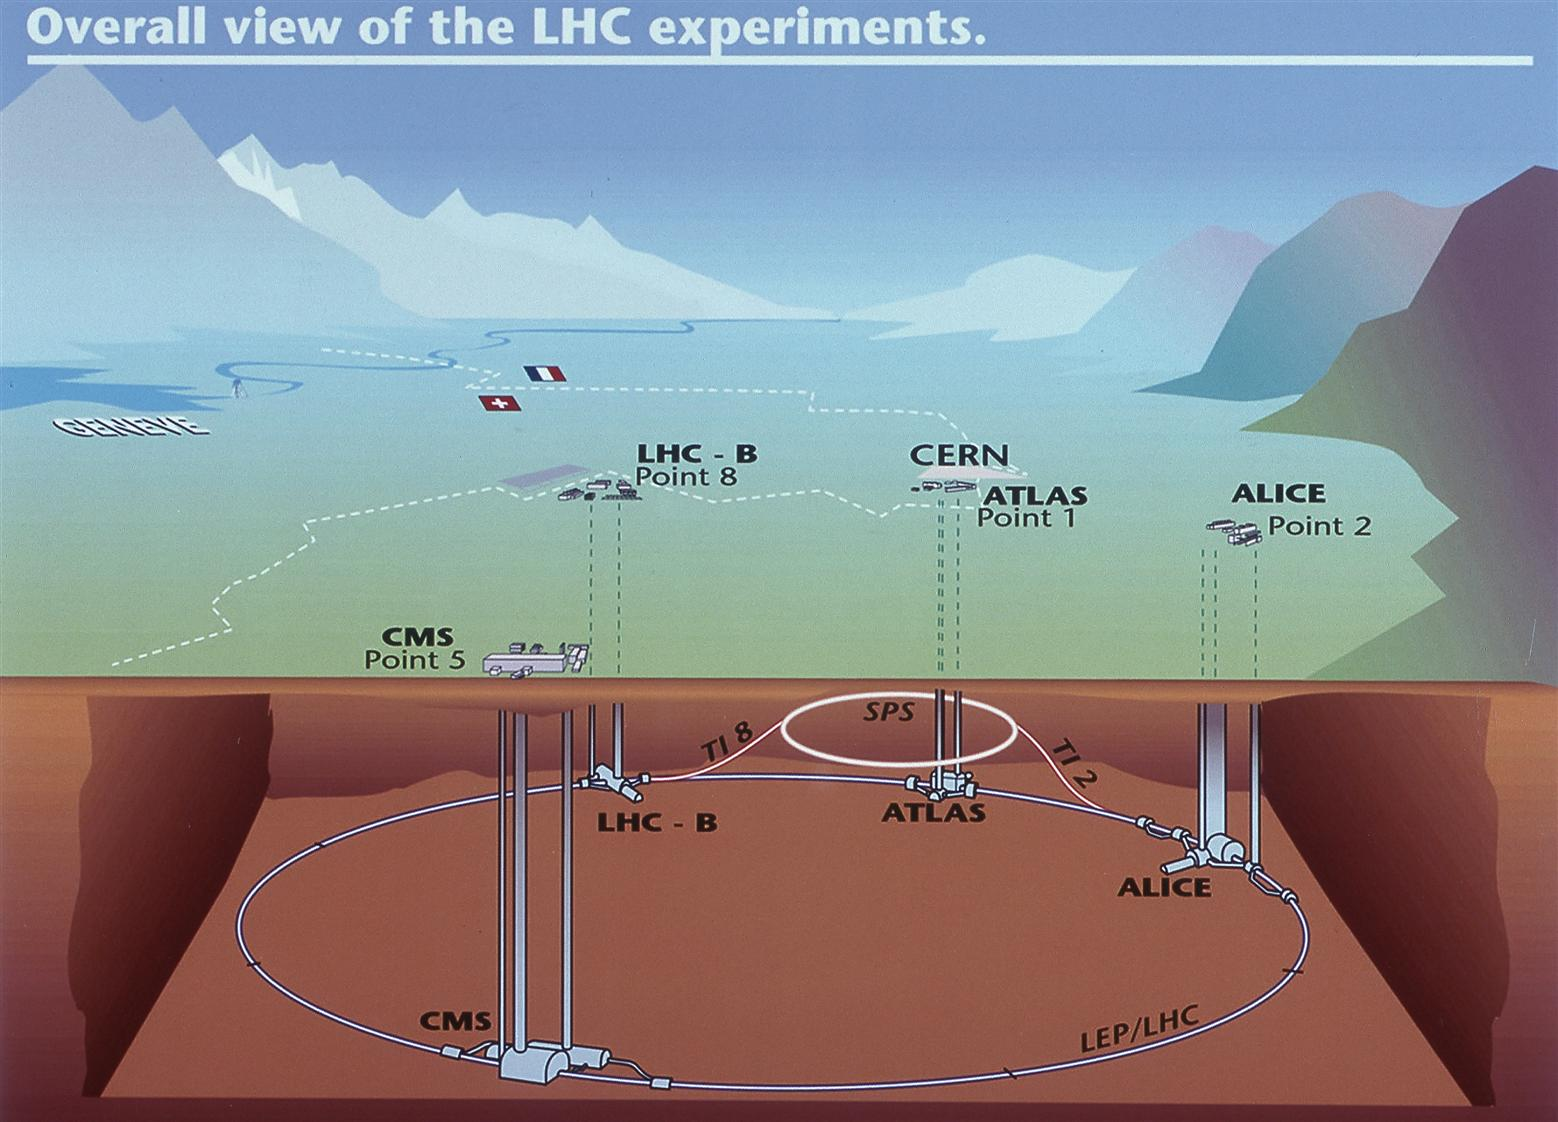
\includegraphics[width=0.9\textwidth]{CERN-all-experiments}
        %\caption{\cite{Pequenao:1095924}}
\end{figure}
\end{column}
\begin{column}{0.5\textwidth}
\begin{itemize}
\item Proton-proton collider
\vspace{0.3cm}
\item $\mysim$ \SI{27}{\kilo \metre} circumfence
\vspace{0.3cm}
\end{itemize}
	     \begin{align*}
	        \hfsetfillcolor{logo_blue!10}
	        \hfsetbordercolor{logo_blue}
	        \tikzmarkin{a1}(0.3,-0.3)(-0.3,0.55)
	        E_{CM} &= \SI{13}{\tera \electronvolt}\\ 
	        \mathcal{L} &= \SI{1.5e34}{\per \square \centi \metre  \per \second} 
	        \tikzmarkend{a1}
	    \end{align*}
\end{column}
\end{columns}
\end{frame}

\begin{frame}{The ATLAS experiment}
    \begin{figure}
        \centering
        \includegraphics[width=0.8\textwidth]{lhc_atlas_combination.eps}
        %\caption{\cite{Pequenao:1095924}}
        \label{fig:my_label}
    \end{figure}
\end{frame}

\begin{frame}{ATLAS - a genereal purpose detector}
    \begin{figure}
        \centering
        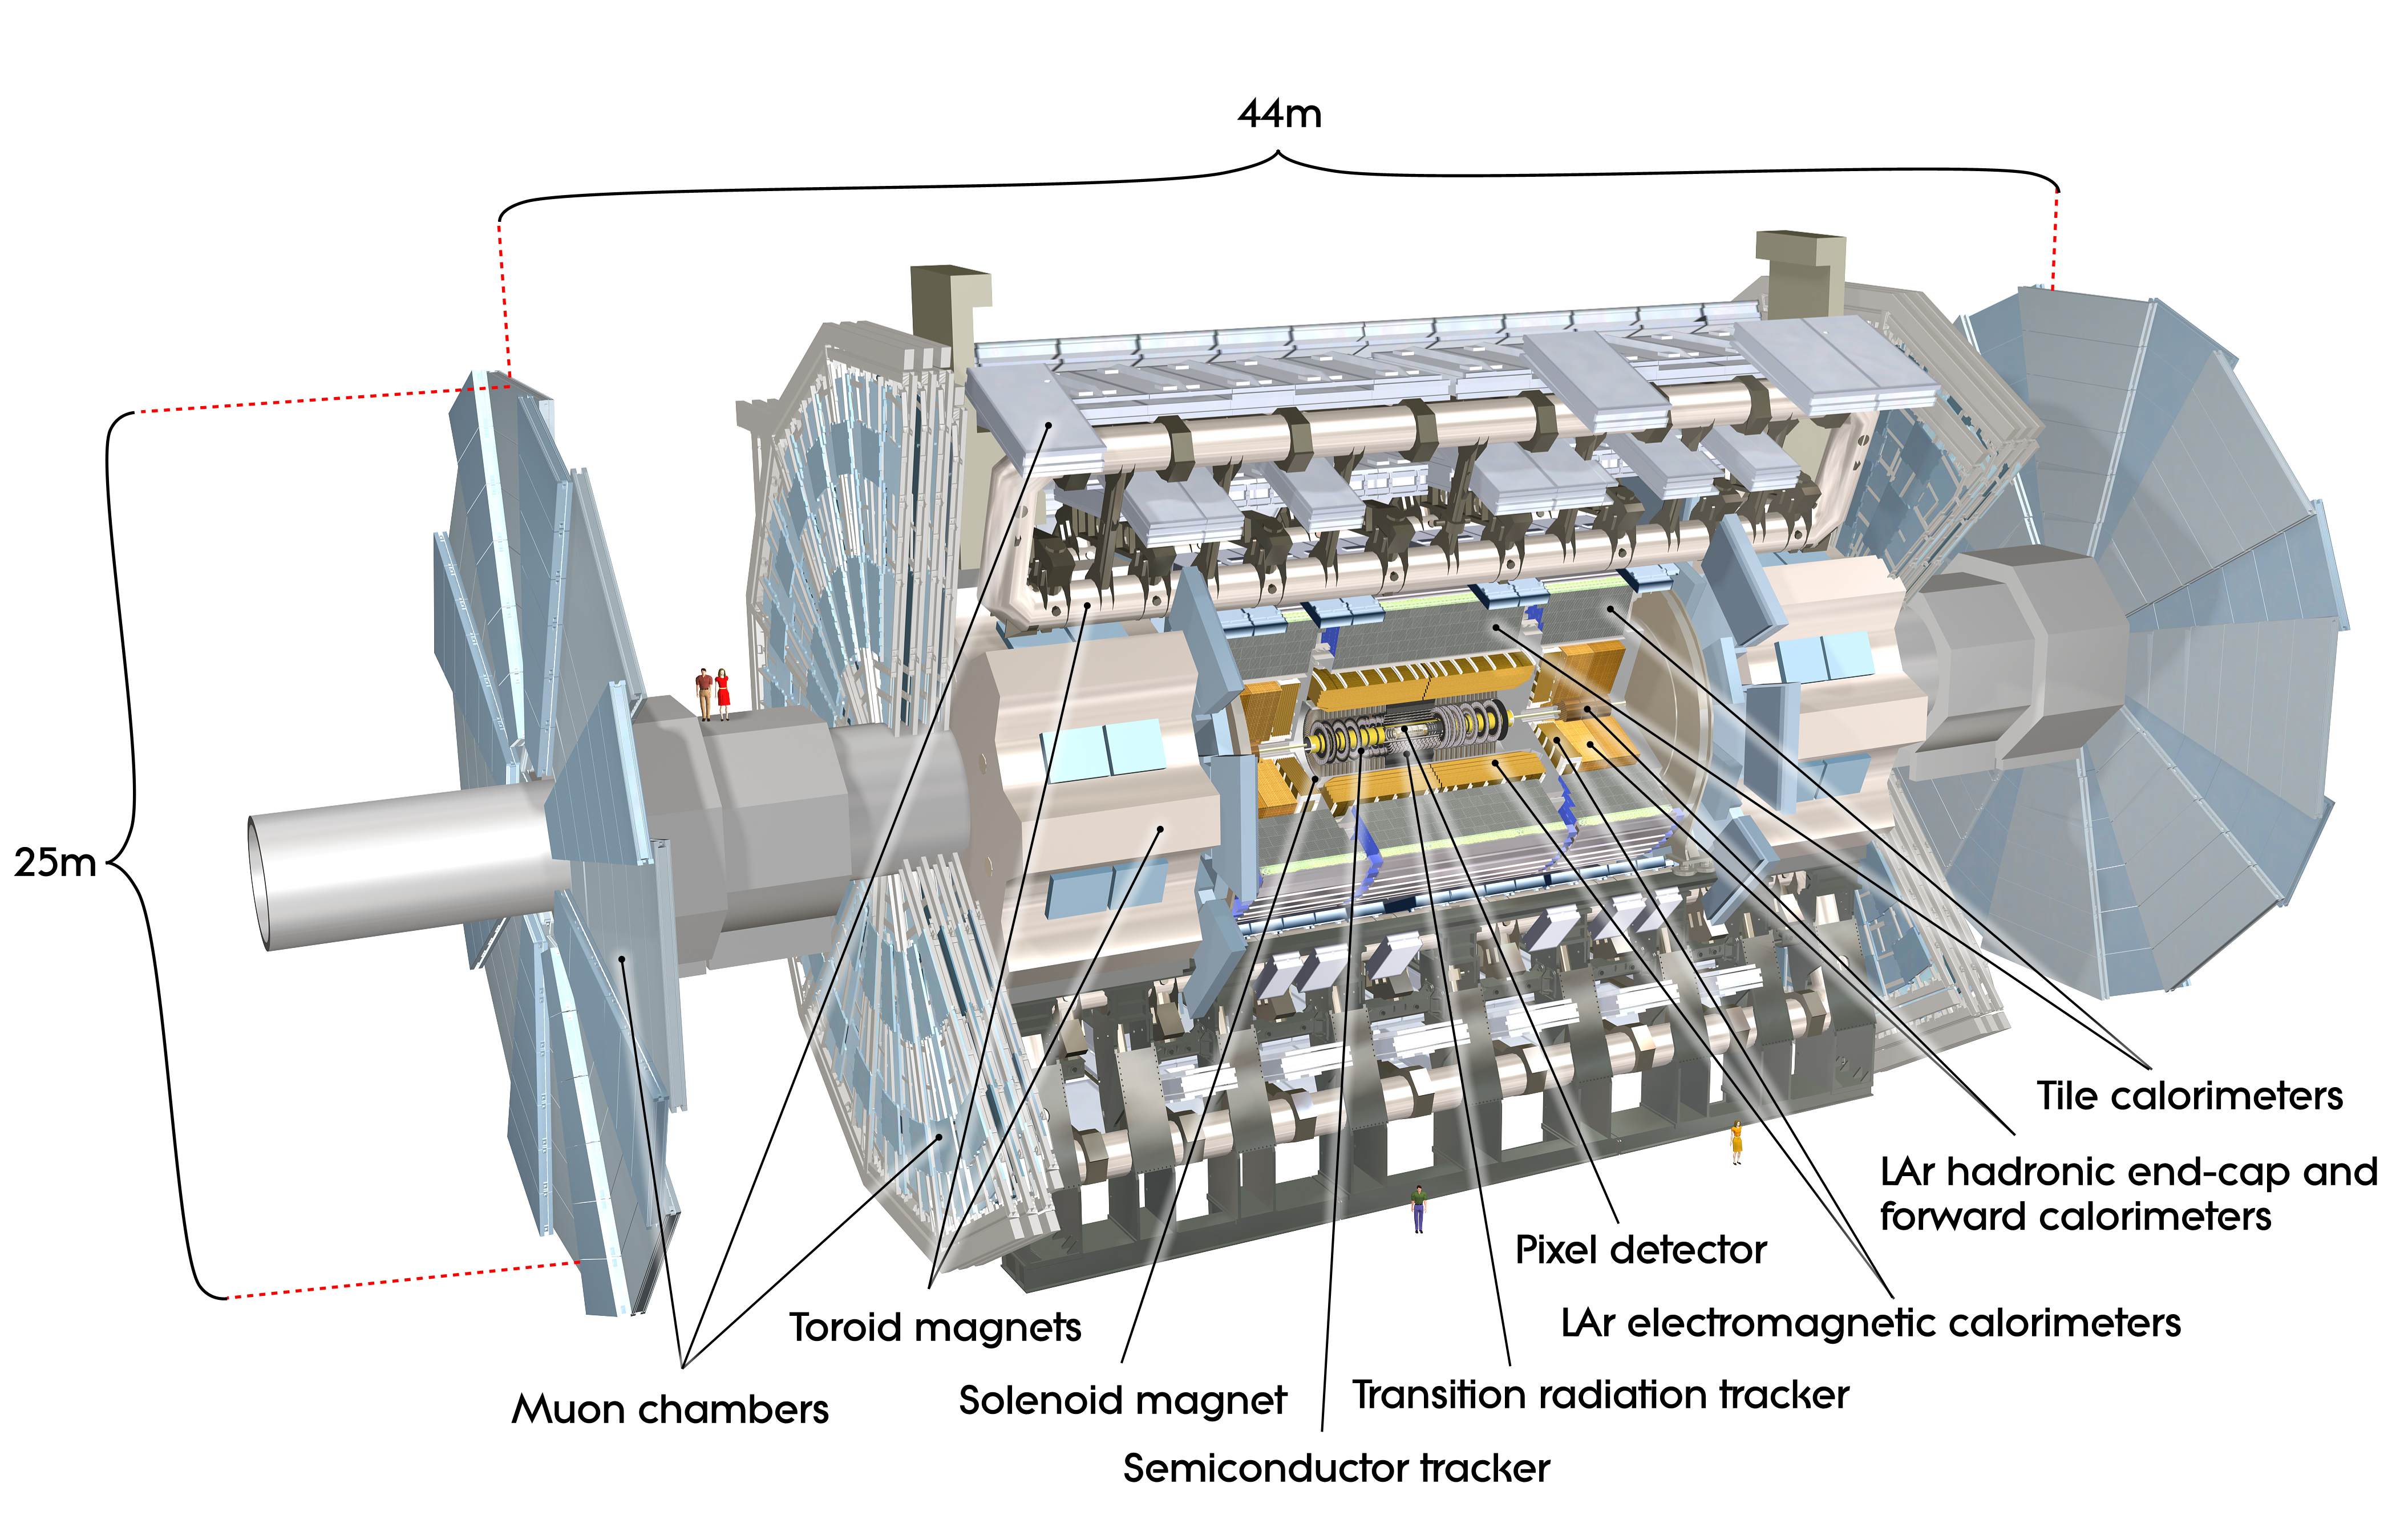
\includegraphics[width=0.8\textwidth]{atlas_detector.jpg}
        %\caption{\cite{Pequenao:1095924}}
        \label{fig:my_label}
    \end{figure}
\end{frame}


\begin{frame}{ATLAS - object identification}
    \begin{figure}
        \centering
        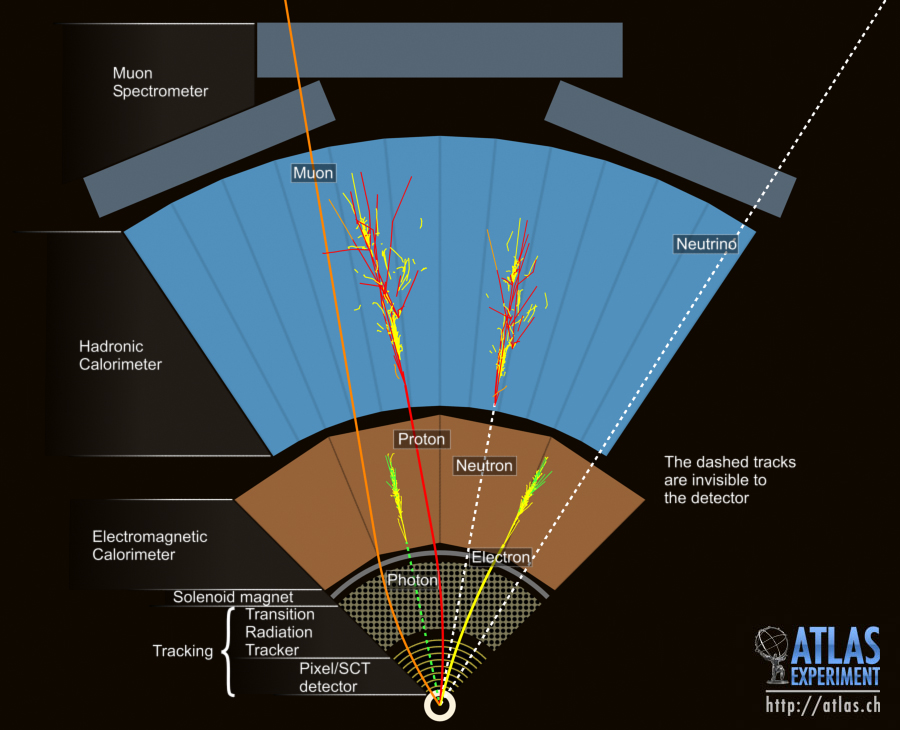
\includegraphics[width=0.8\textwidth]{figures_theory/atlas_quer.jpg}
        %\caption{\cite{Pequenao:1095924}}
        \label{fig:my_label}
    \end{figure}
\end{frame}



\begin{frame}{\tW to \ttbar separation at LO}
\begin{columns}
\quad
    \begin{column}{0.45\textwidth}
    \begin{block}{\tW decay}
    \end{block}
    \end{column}
    \quad
    \begin{column}{0.45\textwidth}
    \begin{block}{\ttbar decay}
    \end{block}
    \end{column}
\quad
\end{columns}
    \begin{figure}[htbp]
    \centering
    \begin{subfigure}[b]{0.4\textwidth}
        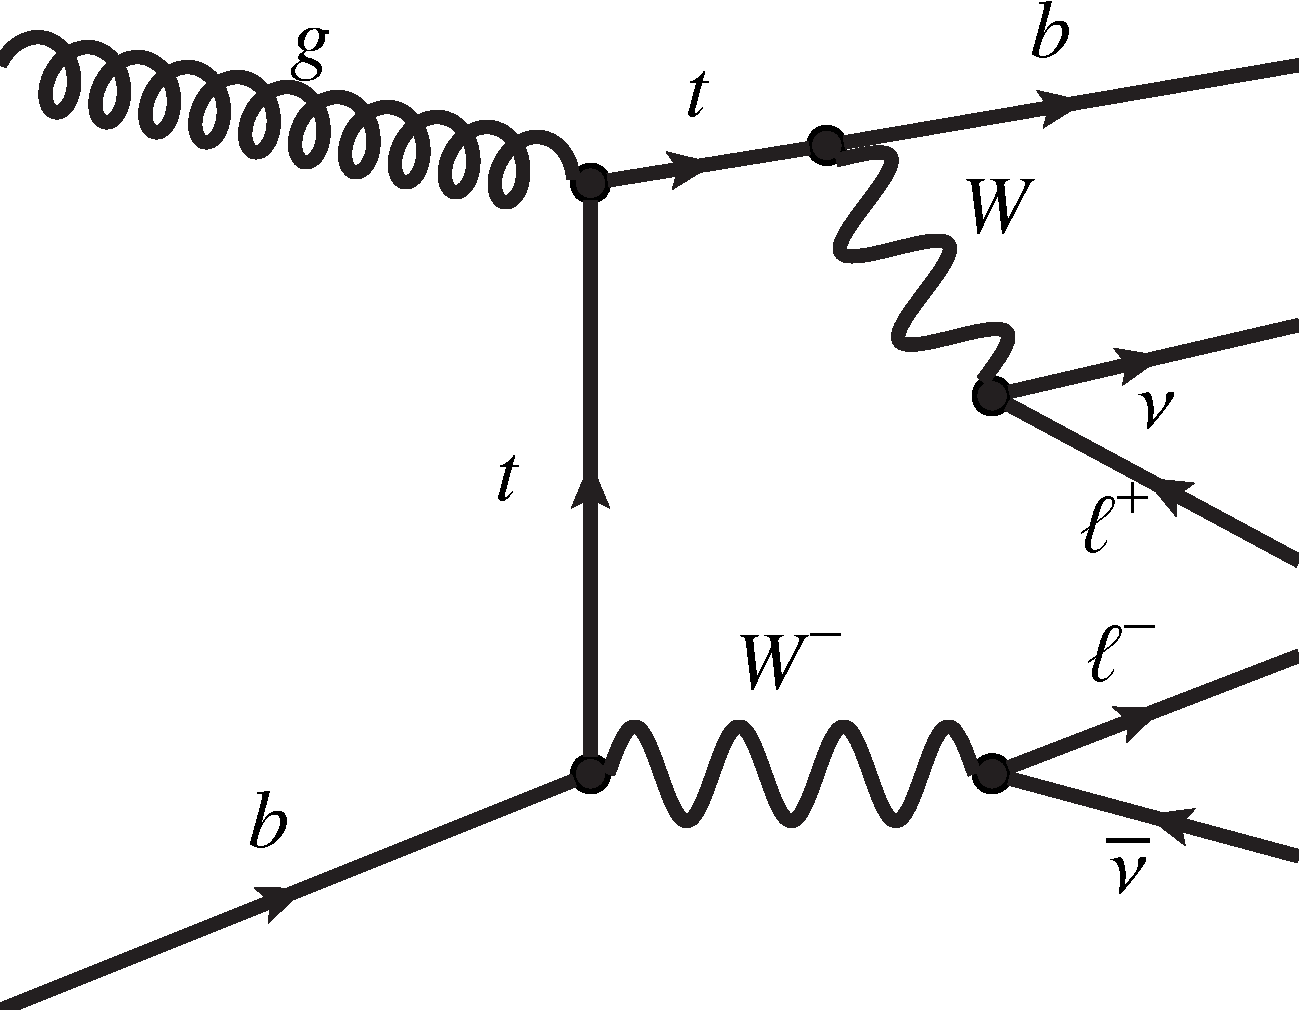
\includegraphics[width=\textwidth]{feynman_diagrams/tW-decay.pdf}
        \label{fig:nlo:tw}
    \end{subfigure}
\quad
    \begin{subfigure}[b]{0.4\textwidth}
        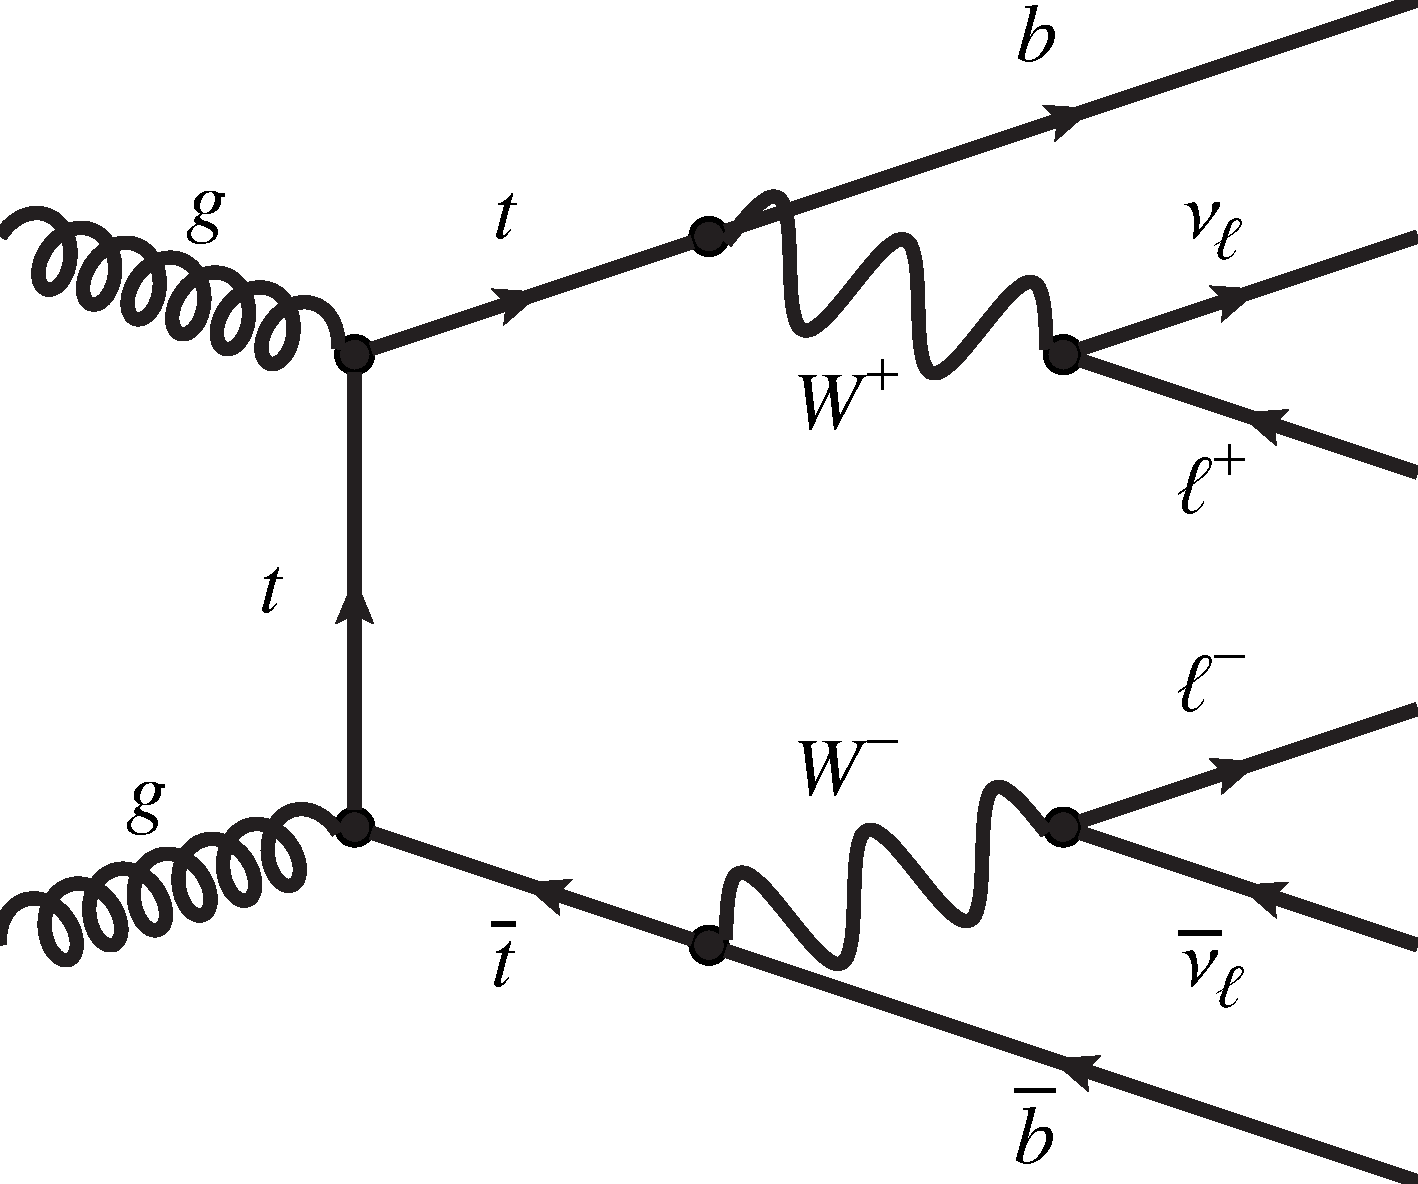
\includegraphics[width=\textwidth]{ttbar-decay}
        \label{fig:nlo:ttbar}
    \end{subfigure}
\end{figure}
\begin{columns}
\quad
    \begin{column}{0.45\textwidth}
	\begin{itemize}
	\item $\sigma_{\tW} \sim \SI{71.7}{\pico\barn}$
	\item 2 \PW, 1 \Pbottom
	\end{itemize}
    \end{column}
    \quad
    \begin{column}{0.45\textwidth}
	\begin{itemize}
	\item $\sigma_{\ttbar} \sim \SI{832}{\pico\barn}$
	\item Final state: 2 \PW, 2 \Pbottom
	\end{itemize}
    \end{column}
\quad
\end{columns}
\end{frame}



\section{Machine Learning}


\begin{frame}{Challenge 1 - Signal to background separation}
\begin{block}{Problem 1}
    \begin{itemize}
        \item Separation of signal to background
        \item Signal: \tW
        \item Background: \ttbar
    \end{itemize}
\end{block}
\begin{block}{Classic approach}
    \begin{itemize}
    \item Applying a cut selection
    \end{itemize}
\end{block}
\begin{block}{Alternative}
    \begin{itemize}
        \item Machine Learning
        \item In particular: Classifying neural network
    \end{itemize}
\end{block}
\end{frame}

\begin{frame}[c]
\begin{center}
\Huge Artificial neural network
\end{center}
\end{frame}

\begin{frame}{Neural Networks - Processing information}
\begin{tabular}{p{5cm}|p{5cm}}
    \begin{figure}
    	
\includegraphics[scale = 0.09]{brain}
    \end{figure}
    & 
    \begin{figure}
    	
\includegraphics[scale = 1.4]{machine}
    \end{figure} \\
  \multicolumn{1}{c|}{Humam senses} & \multicolumn{1}{c}{Input variables} \\
    \begin{itemize}
        \item Extraction of relevant info
        \item Impossible for machines
    \end{itemize}
    & 
    \begin{itemize}
      \item Preprocessed by user
      \item {e.g.} kinematic variables
    \end{itemize} \\
\multicolumn{1}{c|}{Human brain} & \multicolumn{1}{c}{Net of nodes} \\
    \begin{itemize}
        \item Web of neuron cells
        \item Input from surrounding cells
        \item Single combination $\rightarrow$ action
    \end{itemize}
    & 
    \begin{itemize}
      \item Nodes = simple processors
      \item Connected by linear function
      \item Combination forms non-linear model
    \end{itemize} 
 \end{tabular}
\end{frame}


\begin{frame}{Neural network structure}
\begin{figure}
\centering
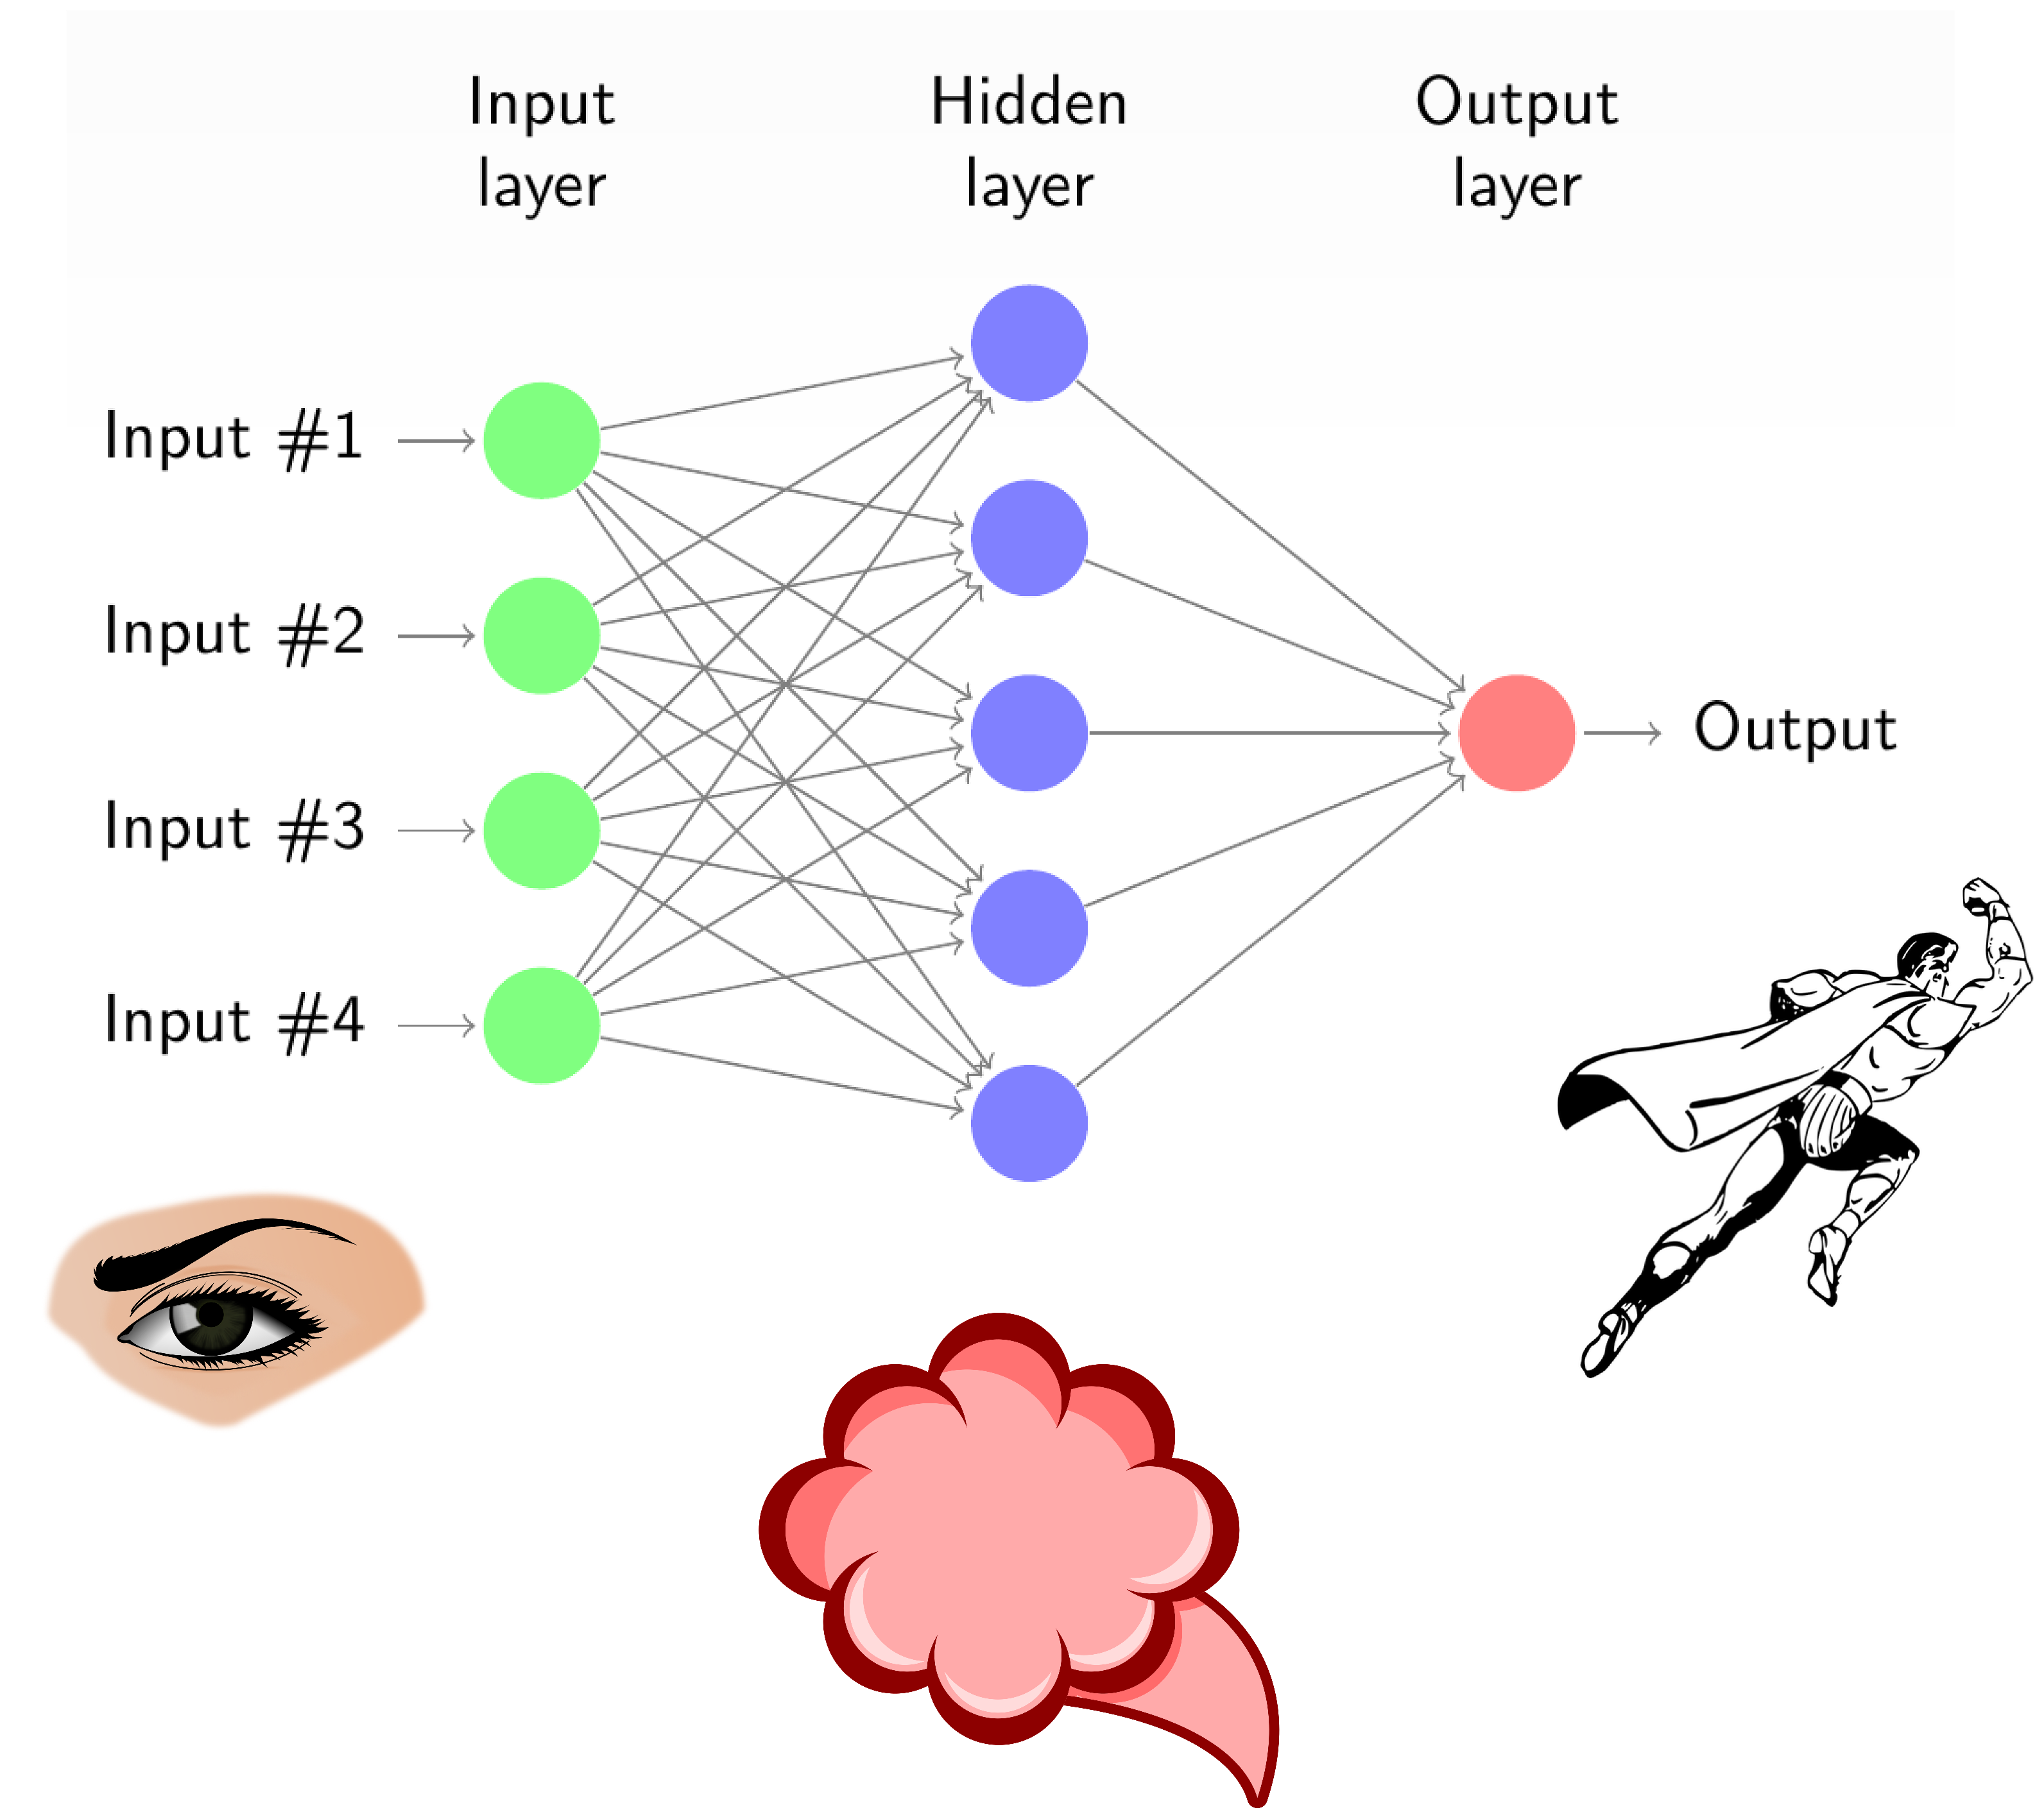
\includegraphics[width=0.8\textwidth]{net_structure}
\end{figure}
\end{frame}

\begin{frame}{Neural Networks - Processing information}
\begin{tabular}{p{5cm}|p{5cm}}
    \begin{figure}
    	
\includegraphics[scale = 0.09]{brain}
    \end{figure}
    & 
    \begin{figure}
    	
\includegraphics[scale = 1.4]{machine}
    \end{figure} \\
  \multicolumn{1}{c|}{Evaluation of an action} & \multicolumn{1}{c}{Loss function} \\
    \begin{itemize}
        \item Simple perceptions: pain, satisfaction
        \item Expectation
    \end{itemize}
    & 
    \begin{itemize}
      \item Supervised learning: compare to the desired outcome
      \item Loss = estimator for quality
    \end{itemize} \\
\multicolumn{1}{c|}{Decision for a next step} & \multicolumn{1}{c}{Optimisation} \\
    \begin{itemize}
        \item Trial and error
        \item Learning from experience
    \end{itemize}
    & 
    \begin{itemize}
      \item Back-propagation impact of parameters' on the loss
      \item Adjust parameters to minimise plot
    \end{itemize} 
 \end{tabular}
\end{frame}



\begin{frame}{Challenge 2 - Sensitivity to systematic uncertainties}
\begin{block}{Problem 2}
    \begin{itemize}
        \item Minimal sensitivity to the systematic uncertainty
        \item Nominal: $\tW\_DR$, (\ttbar)
        \item Systematic: $\tW\_DS$
    \end{itemize}
\end{block}
\begin{block}{Presented solution}
   \begin{itemize}
       \item Addition of a second classifier for nominal to systematics separation
       \item Bad performance $\longrightarrow$ low sensitivity
   \end{itemize}
\end{block}
\begin{block}{Implementation}
    \begin{itemize}
        \item Feed output into a second net
        \item Iterative training
        \item Combined loss function $\longrightarrow$ Minimax problem
    \end{itemize}
\end{block}
\end{frame}

\begin{frame}{Adversarial neural network}
\vspace{-0.3cm}
    \begin{figure}
        \centering
        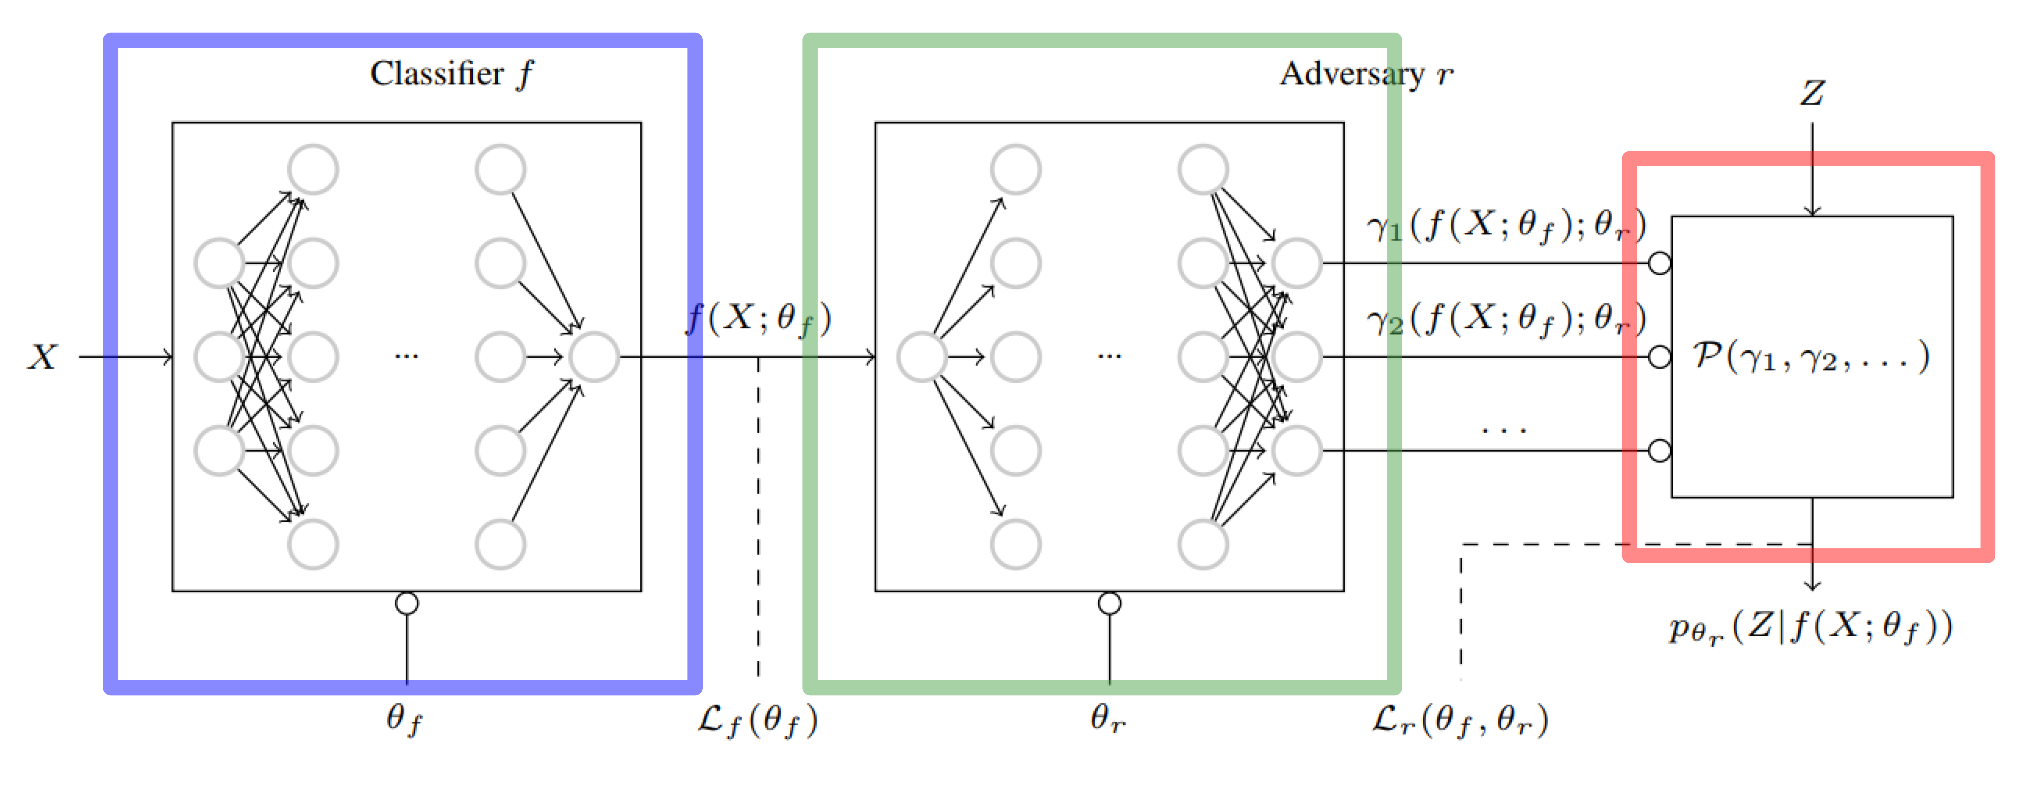
\includegraphics[width=\textwidth]{figures_theory/ANN_paper.eps}
        \caption{(arXiv:1611.01046)}
    \end{figure}
    \begin{equation*}
        \hfsetfillcolor{logo_blue!10}
        \hfsetbordercolor{logo_blue}
        \tikzmarkin{a}(0.3,-0.5)(-0.3,0.55)
        \mathbb{E}(\theta_f, \theta_r) = \mathcal{L}_f(\theta_f) - \lambda \mathcal{L}_r(\theta_f, \theta_r)
        \tikzmarkend{a}
    \end{equation*}
\end{frame}

\begin{frame}{Expected ANN losses}
    \begin{figure}
        \centering
        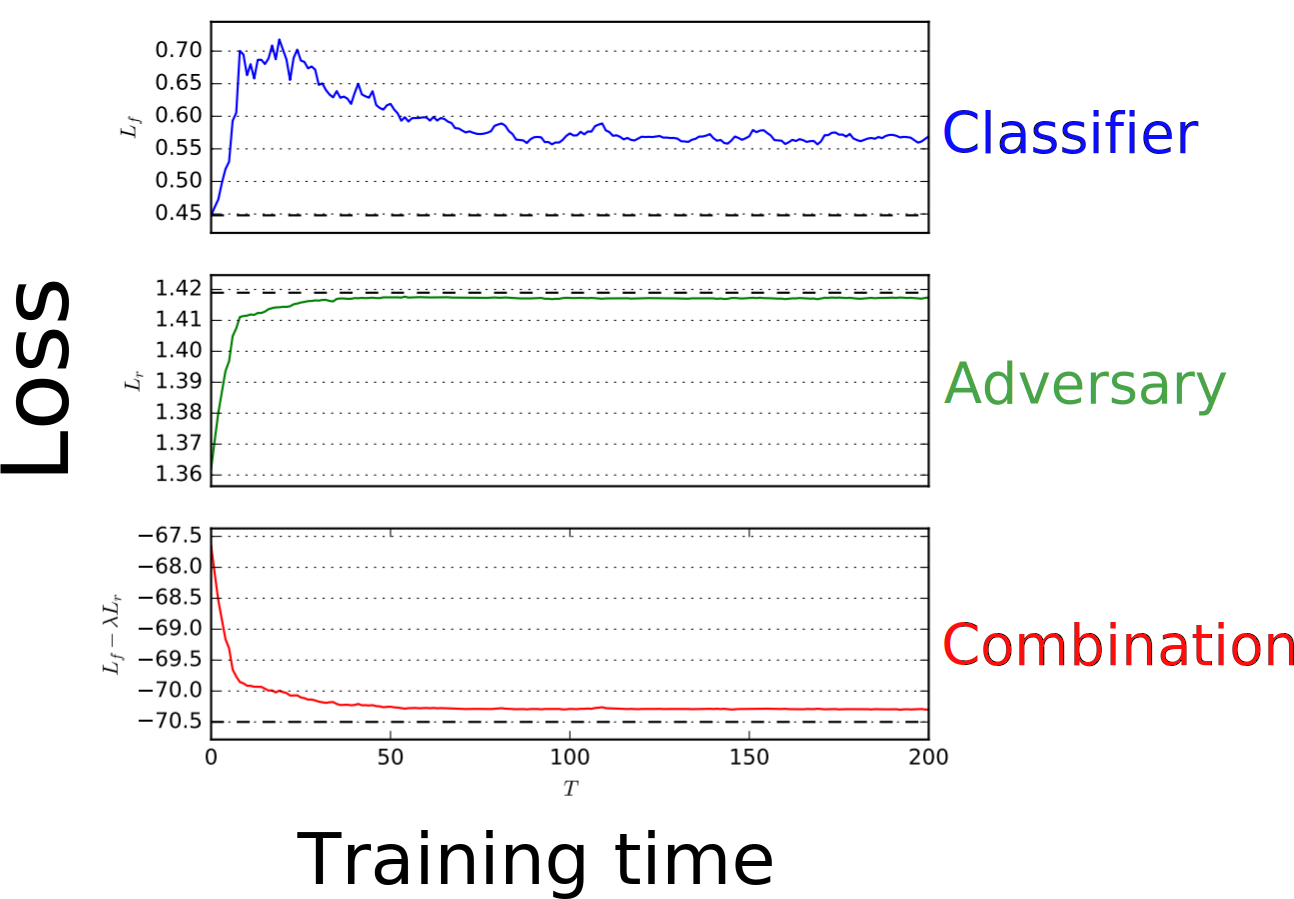
\includegraphics[width=0.9\textwidth]{figures_theory/losses_paper}
        \caption{(arXiv:1611.01046)}
    \end{figure}
\end{frame}
\begin{frame}[c]
\begin{center}
\Huge Classifier training
\end{center}
\end{frame}

\begin{frame}{Setup of the classifier}
\begin{block}{Hyper-parameter scan results}
\begin{itemize}
\item Input: \num{14} variables motivated by a BDT variable scan.
\item Hidden layers: \num{6} \ELU layers $\times$ \num{128} nodes each
\item Output layer: \num{1} \SIGMOID node
\item Optimisation: SGD, \textcolor{red}{learning rate $=0.06$}, momentum $=0.3$, no nesterov, no decay
\item Duration: 600 epochs
\end{itemize}
\end{block}
\end{frame}

\begin{frame}{Simple network results}
\vspace{-2mm}
\begin{figure}[htbp]
    \centering
    \begin{subfigure}[b]{0.4\textwidth}
        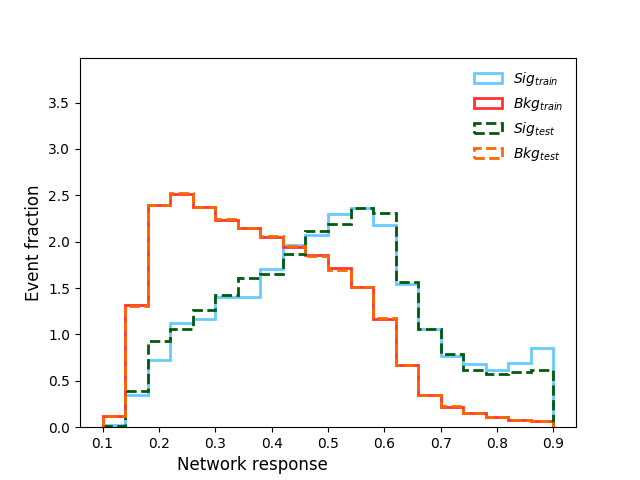
\includegraphics[width=\textwidth]{standard_separation}
        \caption{Separation}
        \label{fig:simple:final:sepa}
    \end{subfigure}
\quad
    \begin{subfigure}[b]{0.4\textwidth}
        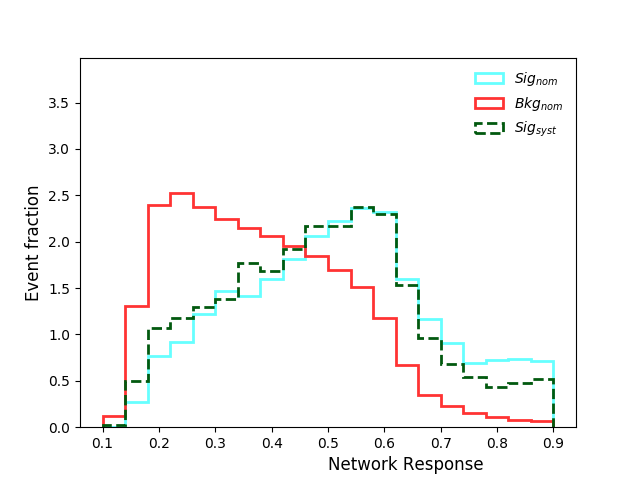
\includegraphics[width=\textwidth]{standard_syst}
        \caption{Systematics}
        \label{fig:simple:final:syst}
    \end{subfigure}

    \begin{subfigure}[b]{0.4\textwidth}
		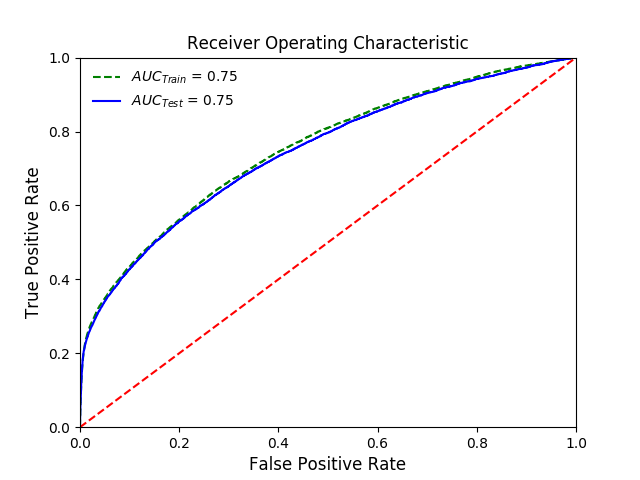
\includegraphics[width=\textwidth]{standard_ROC}
		\caption{ROC curve}
		\label{fig:simple:final:roc}
	\end{subfigure}
\quad
	\begin{subfigure}[b]{0.4\textwidth}
		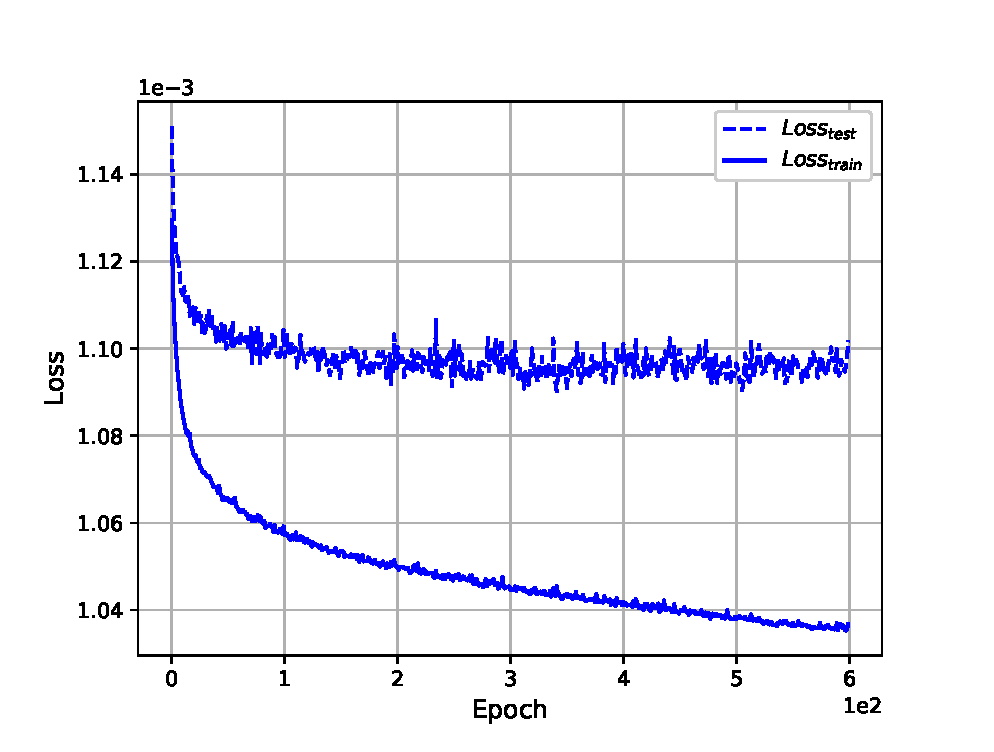
\includegraphics[width=\textwidth]{standard_losses}
		\caption{Losses}
		\label{fig:simple:final:loss}
	\end{subfigure}
\end{figure}
\end{frame}
\begin{frame}{\tW to \ttbar separation at NLO}
\begin{columns}
\quad
    \begin{column}{0.45\textwidth}
    \begin{block}{\tW decay at NLO}
    \end{block}
    \end{column}
    \quad
    \begin{column}{0.45\textwidth}
    %
    \begin{block}{\ttbar decay}
    \end{block}
    \end{column}
\quad
\end{columns}
    \begin{figure}[htbp]
    \centering
    \begin{subfigure}[b]{0.44\textwidth}
        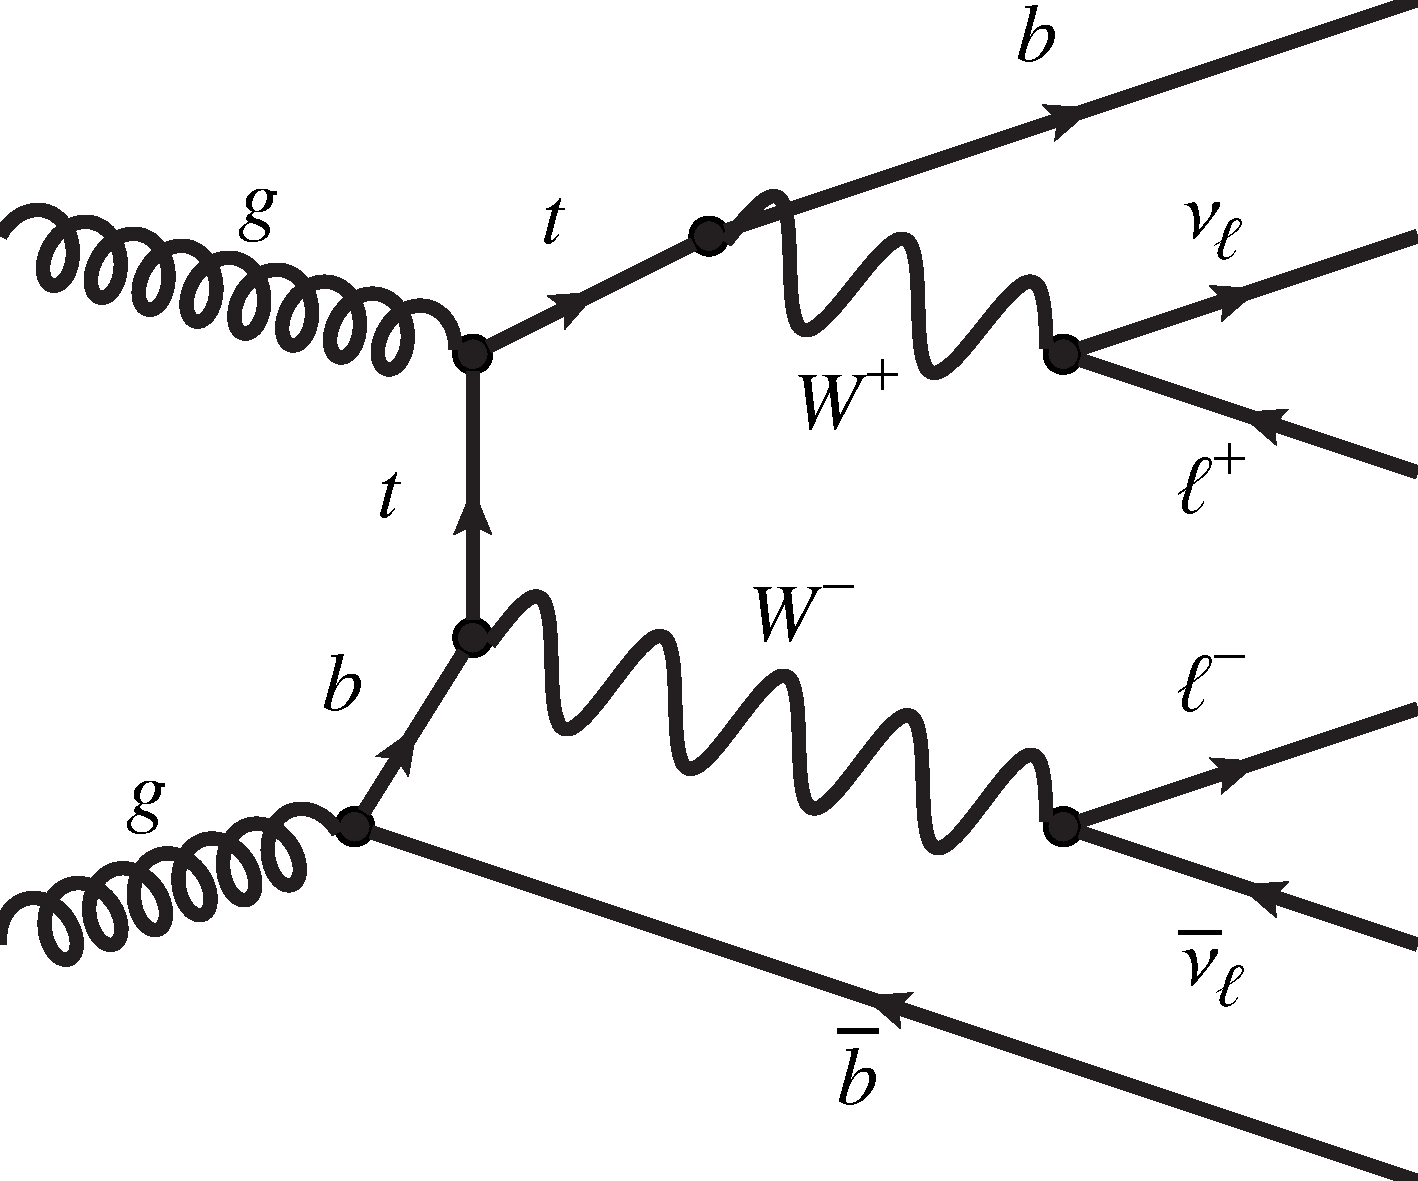
\includegraphics[width=\textwidth]{feynman_diagrams/tw-NLO.pdf}
        %\caption{}
        \label{fig:nlo:ttbar}
    \end{subfigure}
\quad
    \begin{subfigure}[b]{0.44\textwidth}
        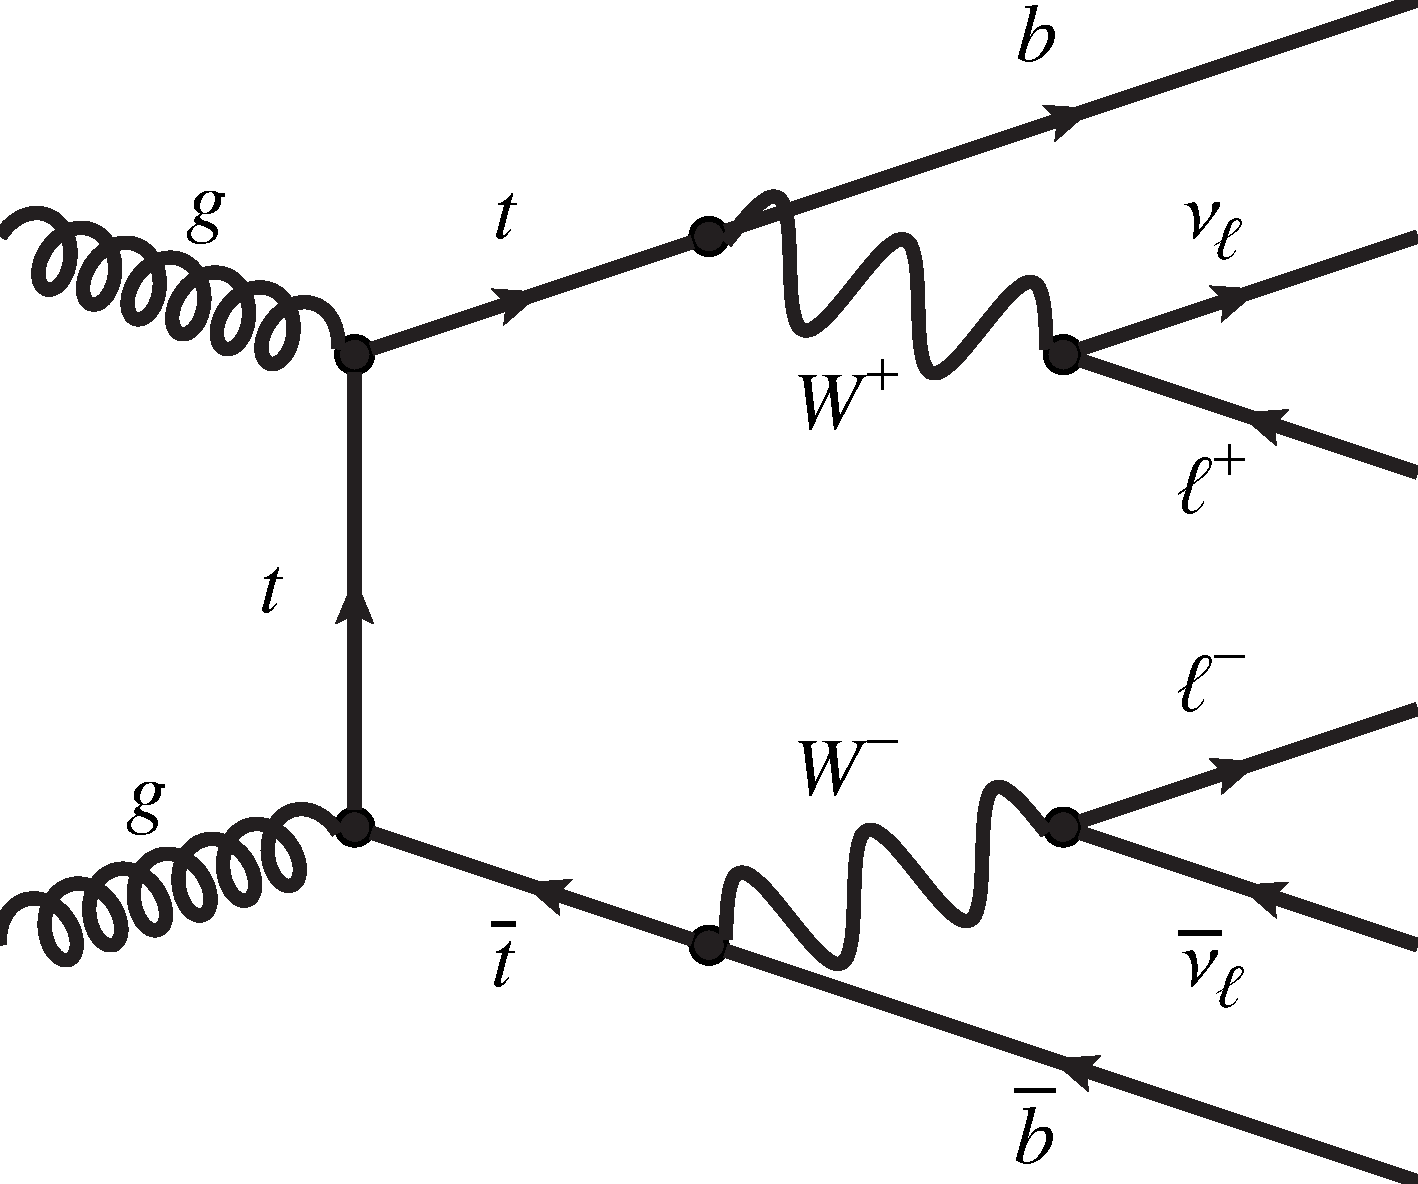
\includegraphics[width=\textwidth]{ttbar-decay}
        %\caption{}
        \label{fig:nlo:tw}
    \end{subfigure}
\end{figure}
%
\begin{columns}
\quad
    \begin{column}{0.45\textwidth}
\begin{itemize}
\item Identical final state
\item Especially problematic in 2j2b region
\end{itemize}
    \end{column}
    \quad
    \begin{column}{0.45\textwidth}
    %
\begin{itemize}
\item Interference at NLO
\item Different Monte Carlo generators
\end{itemize}
    \end{column}
\quad
\end{columns}
\end{frame}

\begin{frame}{Interference in Monte Carlo}
\begin{block}{Amplitude}
\vspace{-0.3cm}
\begin{align*}
|\Aamp|^2 &= |\Atw|^2 + 2 \mathcal{R} \{ \Atw \Att^{\ast} \} + |\Att|^2, \\
&\equiv \Samp + \Iamp + \Damp.
\end{align*}
\end{block}
\begin{block}{Diagram Removal - DR}
\vspace{-0.3cm}
\begin{align*}
| \ADR |^2 = \Samp.
\end{align*}
\end{block}
\begin{block}{Diagram Subtraction - DS}
\vspace{-0.3cm}
\begin{align*}
| \ADS |^2 &= \Samp + \Iamp + \Damp - \widetilde{\Damp},\\
&\approx \Samp + \Iamp.
\end{align*}
\end{block}
\end{frame}

\begin{frame}{Sensitivity to systematic uncertainty}
\vspace{-0.2cm}
\begin{figure}
        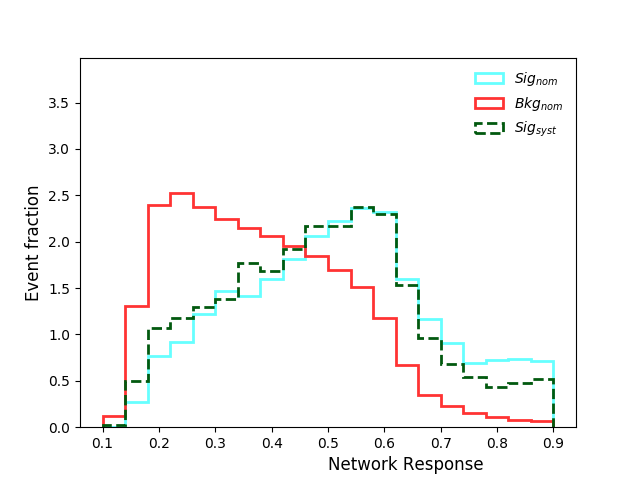
\includegraphics[width=0.8\textwidth]{standard_syst}
%        \caption{Response divided by sample}
%        \label{fig:simple:final:syst}
\end{figure}
\end{frame}

\begin{frame}[c]
\begin{center}
\Huge Adversarial Neural Network
\end{center}
\end{frame}

\begin{frame}{Challenge 2 - Sensitivity to systematic uncertainties}
\begin{block}{Problem 2}
    \begin{itemize}
        \item Minimal sensitivity to the systematic uncertainty
        \item Nominal: $\tW\_DR$, (\ttbar)
        \item Systematic: $\tW\_DS$
    \end{itemize}
\end{block}
\begin{block}{Presented solution}
   \begin{itemize}
       \item Addition of a second classifier for nominal to systematics separation
       \item Bad performance $\longrightarrow$ low sensitivity
   \end{itemize}
\end{block}
\begin{block}{Implementation}
    \begin{itemize}
        \item Feed output into a second net
        \item Iterative training
        \item Combined loss function $\longrightarrow$ Minimax problem
    \end{itemize}
\end{block}
\end{frame}

\begin{frame}{Adversarial neural network}
\vspace{-0.3cm}
    \begin{figure}
        \centering
        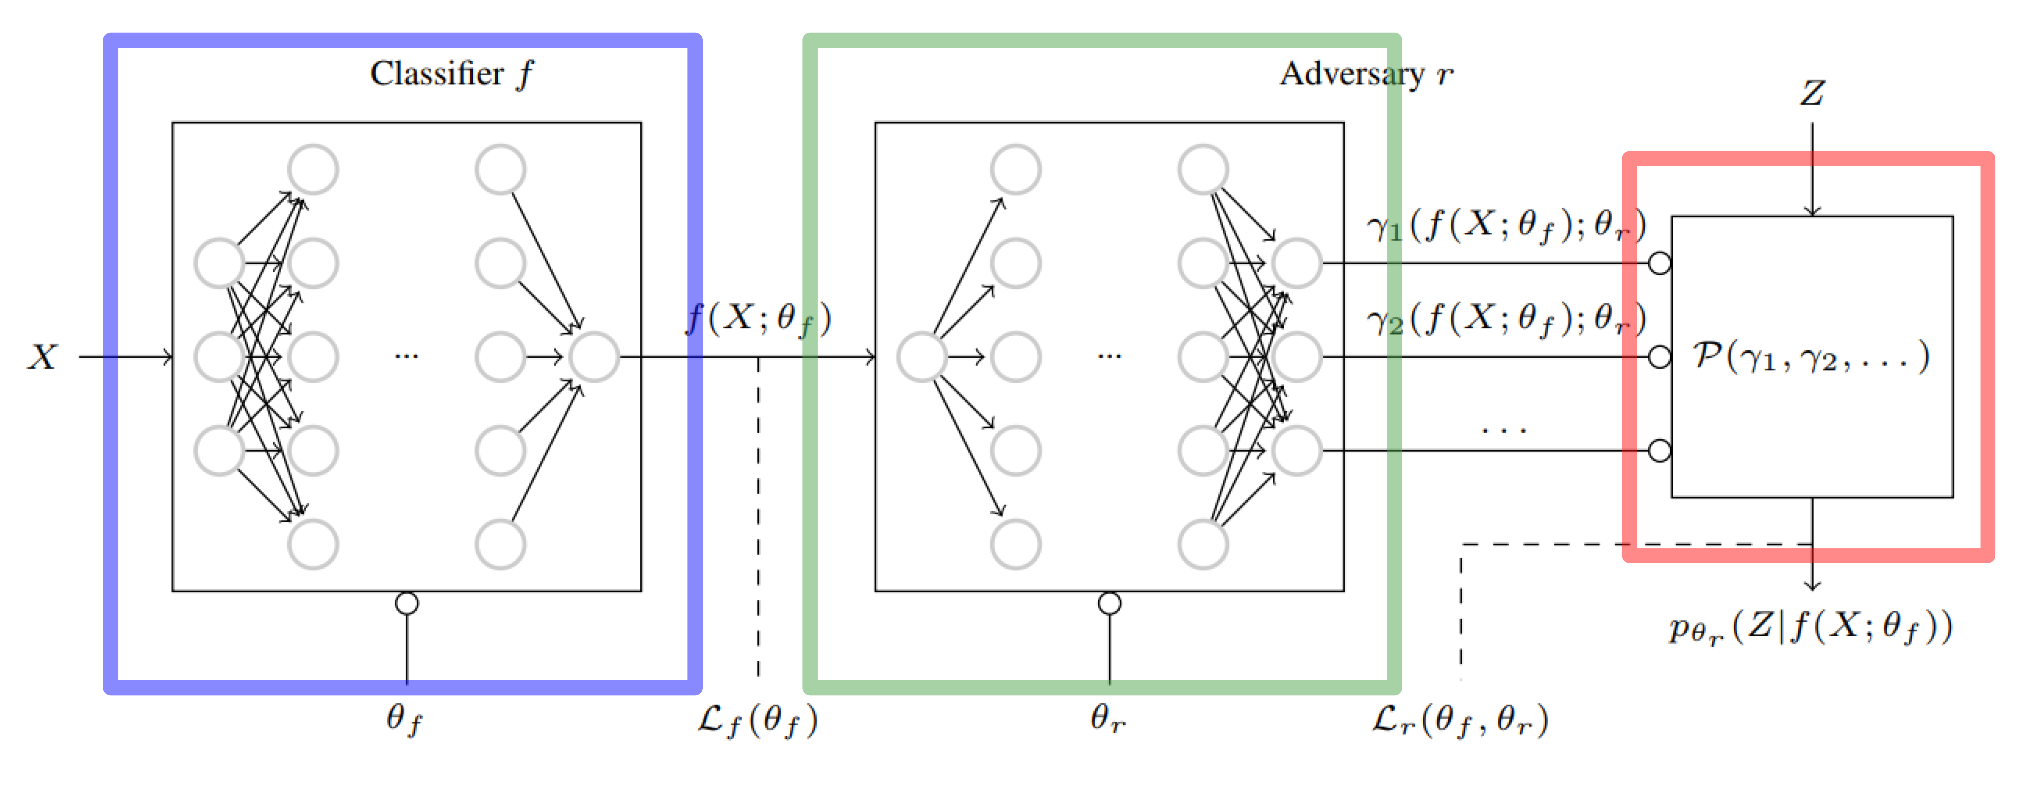
\includegraphics[width=\textwidth]{figures_theory/ANN_paper.eps}
        \caption{(arXiv:1611.01046)}
    \end{figure}
    \begin{equation*}
        \hfsetfillcolor{logo_blue!10}
        \hfsetbordercolor{logo_blue}
        \tikzmarkin{a}(0.3,-0.5)(-0.3,0.55)
        \mathbb{E}(\theta_f, \theta_r) = \mathcal{L}_f(\theta_f) - \lambda \mathcal{L}_r(\theta_f, \theta_r)
        \tikzmarkend{a}
    \end{equation*}
\end{frame}

\begin{frame}{Expected ANN losses}
    \begin{figure}
        \centering
        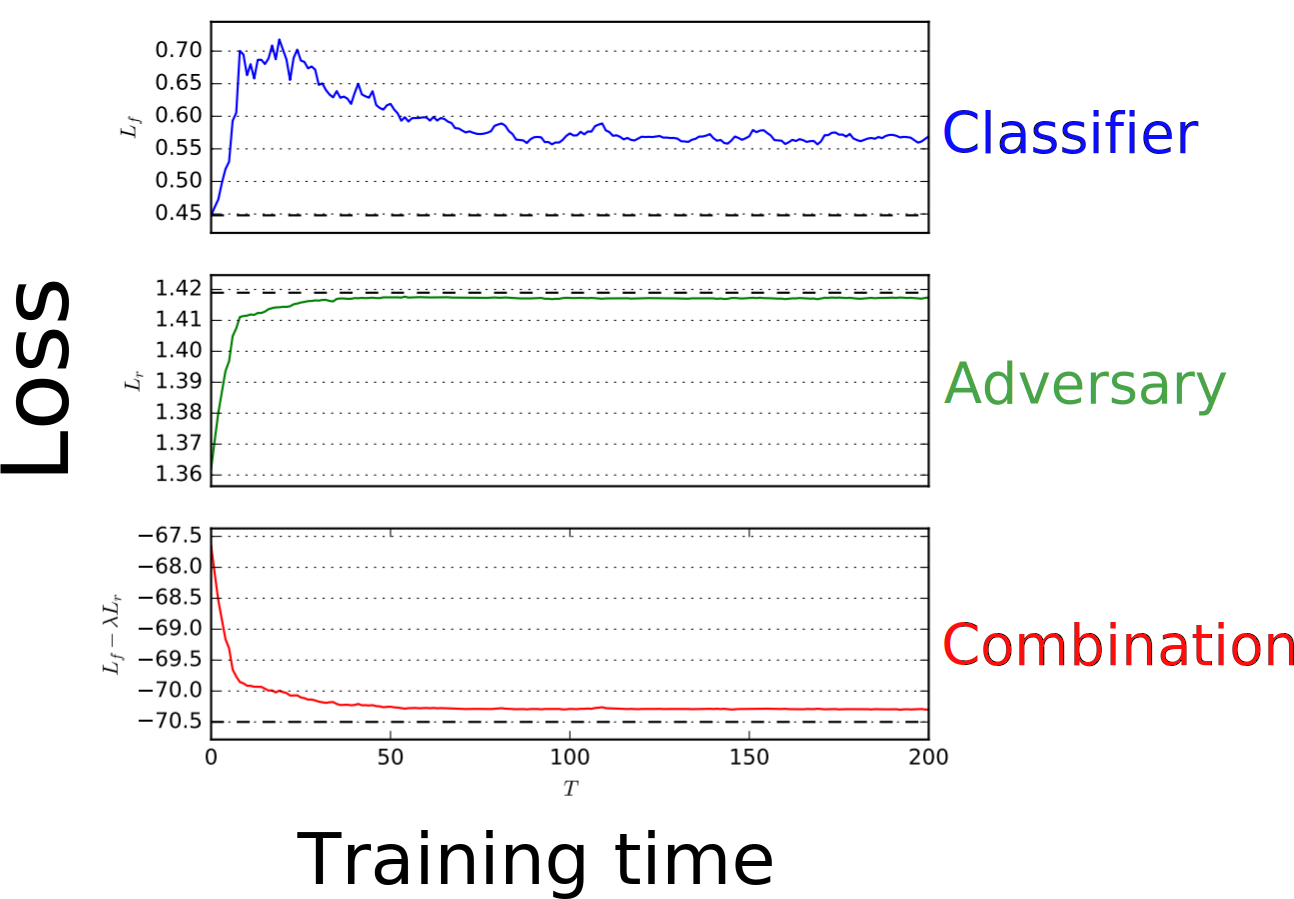
\includegraphics[width=0.9\textwidth]{figures_theory/losses_paper}
        \caption{(arXiv:1611.01046)}
    \end{figure}
\end{frame}
\section{Results}






\begin{frame}[c]
\begin{center}
\Huge Adversarial training
\end{center}
\end{frame}

\begin{frame}{Approach 1}
    \begin{block}{Run 1}
\begin{itemize}
    \item Same hyper-parameters for both networks
    \item Adversary uses only 3 layers
\end{itemize}
    \end{block}
    \begin{block}{Setup}
    \begin{itemize}
    \item Input: \num{14} variables motivated by a BDT variable scan.
    \item Hidden layers: \num{3}(\num{6}) \ELU layers $\times$ \num{128} nodes each
    \item Output layer: \num{1} \SIGMOID node
    \item Optimisation: SGD, Learning rate $=0.06$, momentum $=0.3$, no nesterov, no decay
    \item Duration: 400 iteration
    \item $\lambda = 10$
    \end{itemize}
    \end{block}
\end{frame}

\begin{frame}{Approach 1 - Run 1 - Results}
    \begin{figure}[htbp]
    \centering
    \begin{subfigure}[b]{0.47\textwidth}
        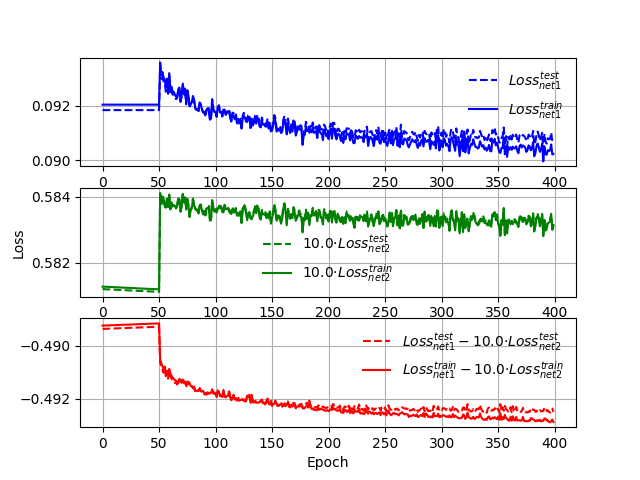
\includegraphics[width=\textwidth]{app1/full_classic_losses.png}
        %\caption{}
        \label{fig:simple:final:sepa}
    \end{subfigure}
\quad
    \begin{subfigure}[b]{0.47\textwidth}
        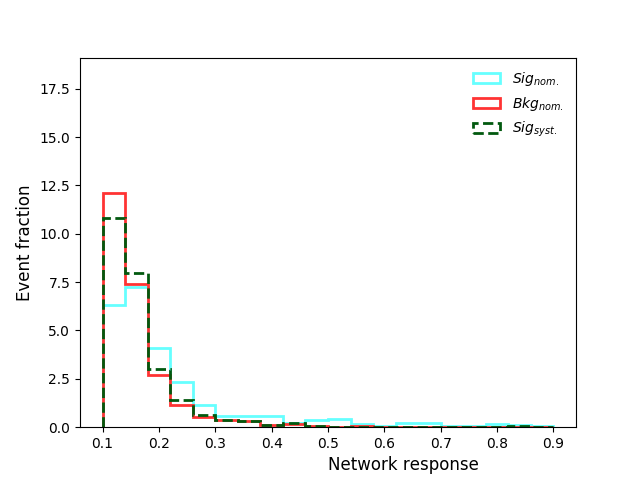
\includegraphics[width=\textwidth]{app1/full_classic_syst.png}
        %\caption{}
        \label{fig:simple:final:syst}
    \end{subfigure}
    \end{figure}
    \begin{itemize}
        \item Both losses decreasing
        \item Only combined losses depend on $\lambda$
        \item Bad separation
        \item High sensitivity to systematics
    \end{itemize}
\end{frame}

\begin{frame}{Approach 1 - Optimisation}
\begin{block}{Setup of the adversary}
    \begin{itemize}
    \item Input: \num{14} variables motivated by a BDT variable scan.
    \item Hidden layers: \num{3} \ELU layers $\times$ \num{32} nodes each
    \item Output layer: \num{1} \SIGMOID node
    \item Optimisation: SGD, Learning rate $=0.001$, momentum $=0.$, no nesterov, no decay
    \item Duration: 400 iteration
    \item $\lambda = 0.1$
    \end{itemize}
    \end{block}
\end{frame}

\begin{frame}{Approach 1 - Run 2 - Results}
    \begin{figure}[htbp]
    \centering
    \begin{subfigure}[b]{0.47\textwidth}
        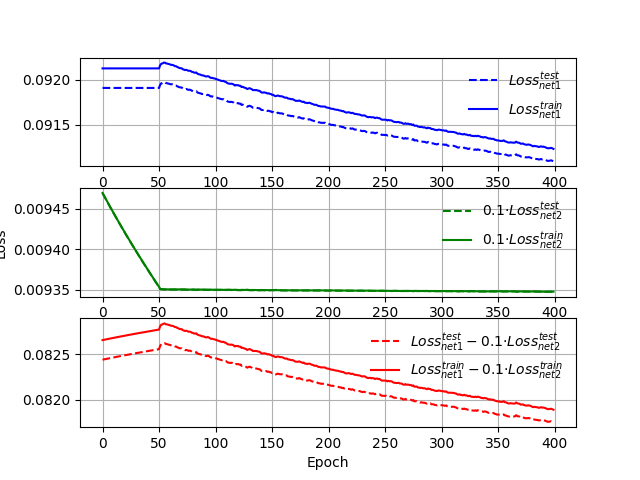
\includegraphics[width=\textwidth]{app1/half_classic_losses.png}
        %\caption{}
        \label{fig:simple:final:sepa}
    \end{subfigure}
\quad
    \begin{subfigure}[b]{0.47\textwidth}
        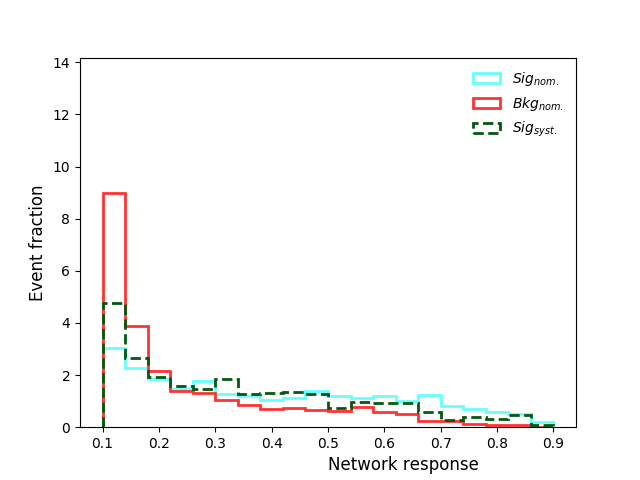
\includegraphics[width=\textwidth]{app1/half_classic_syst.png}
        %\caption{}
        \label{fig:simple:final:syst}
    \end{subfigure}
    \end{figure}
    \begin{itemize}
        \item Visible separation
        \item Adversary loss stops falling
        \item No improvement in the sensitivity visible
    \end{itemize}
\end{frame}

\begin{frame}{Approach 2}
\begin{figure}
    \centering
    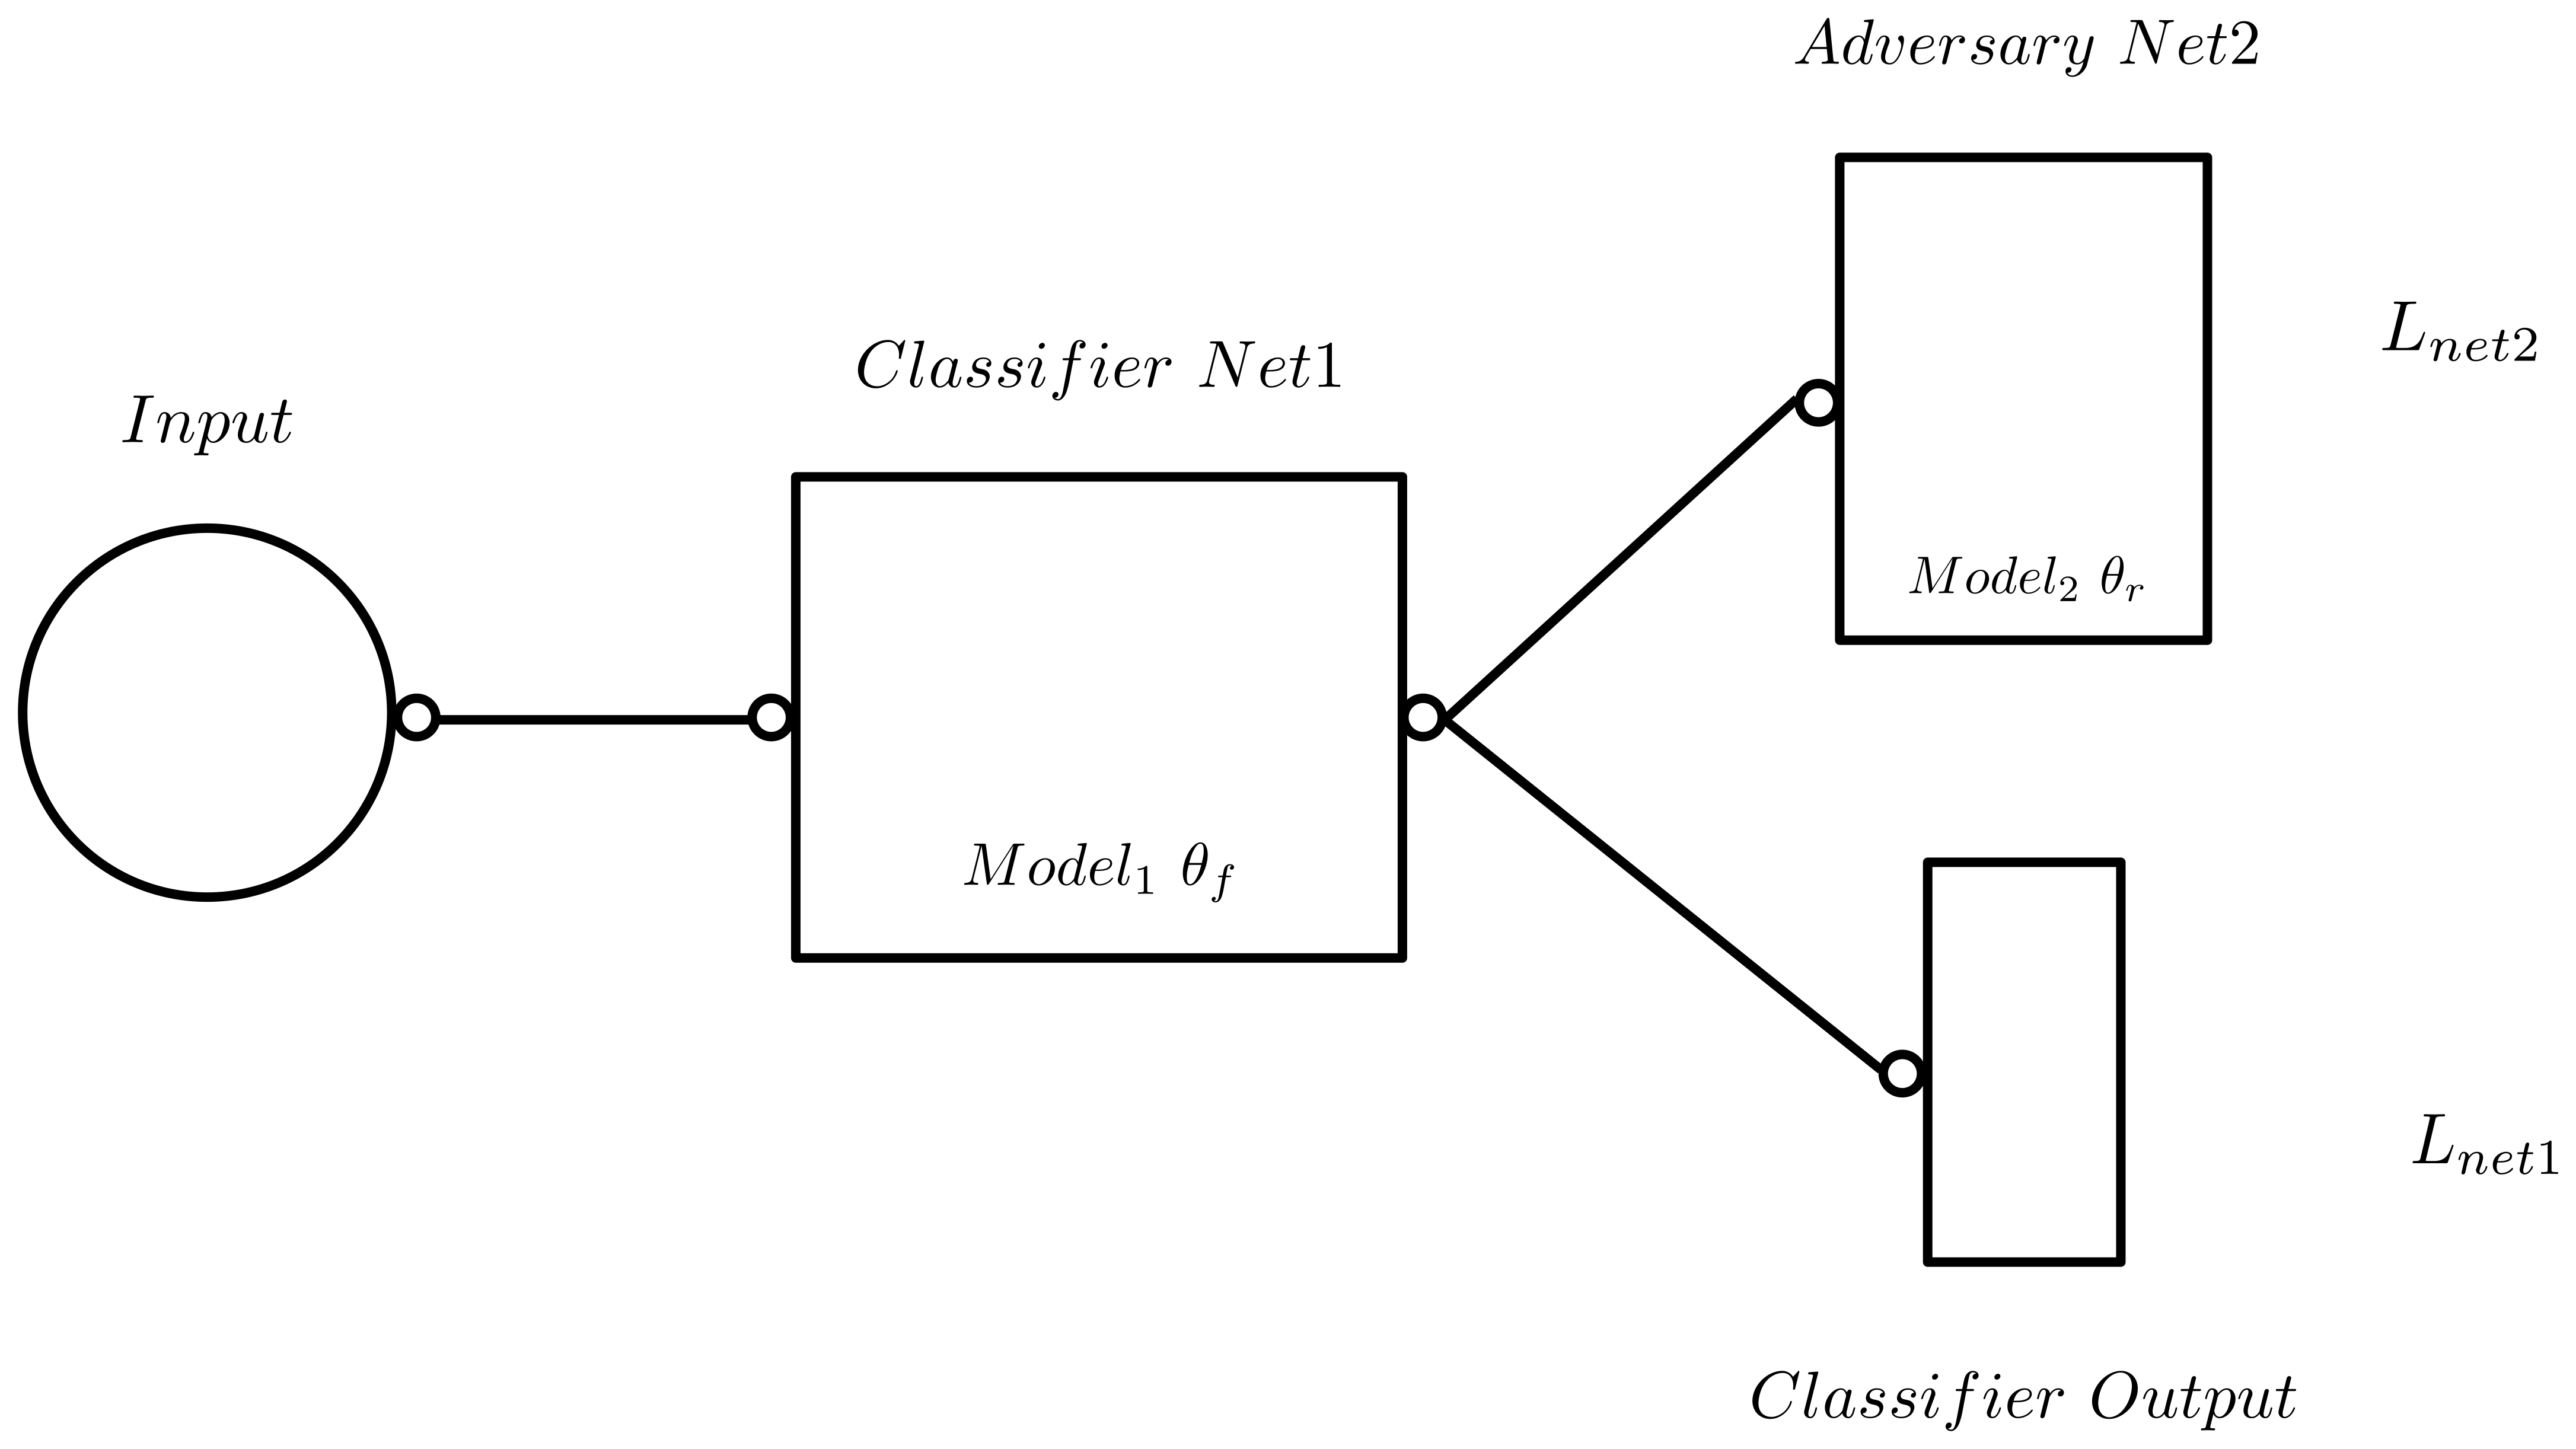
\includegraphics[width=0.8\textwidth]{figures_theory/ANN_sketch.png}
    %\caption{Caption}
\end{figure}
    \begin{block}{Input the last hidden layer to the adversary}
        \begin{itemize}
            \item More information provided
            \item Possible danger: Missing last decision step
        \end{itemize}
    \end{block}
\end{frame}


\begin{frame}{Approach 2 Results}
    \begin{figure}[htbp]
    \centering
    \begin{subfigure}[b]{0.47\textwidth}
        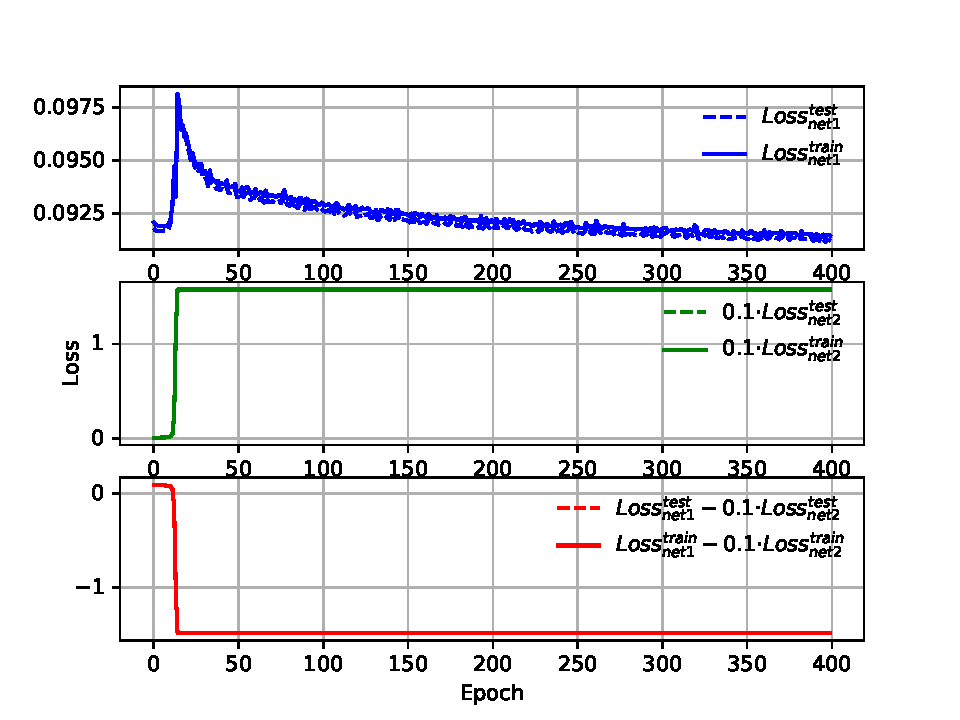
\includegraphics[width=\textwidth]{app2/app2_losses2.pdf}
        %\caption{}
        \label{fig:simple:final:sepa}
    \end{subfigure}
\quad
    \begin{subfigure}[b]{0.47\textwidth}
        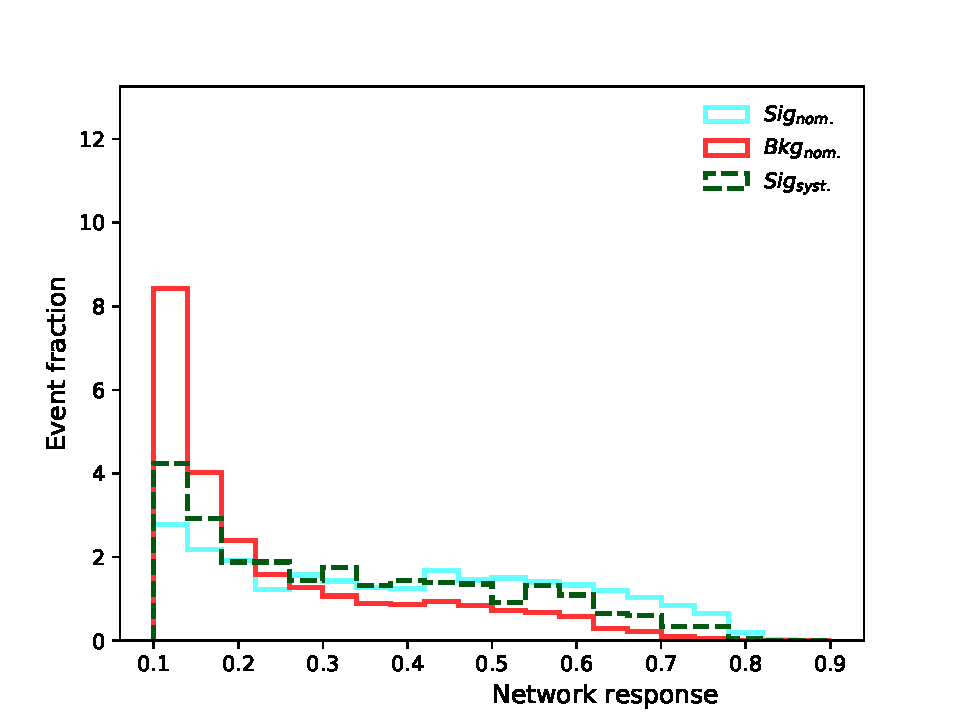
\includegraphics[width=\textwidth]{app2/app2_syst.pdf}
        %\caption{}
        \label{fig:simple:final:syst}
    \end{subfigure}
    \end{figure}
        \begin{itemize}
            \item Losses behave as desired
            \item steep rise, although partially due to scale
            \item $\lambda$ almost unusable due to difference in magnitude
            \item still high sensitivity
        \end{itemize}
\end{frame}

\begin{frame}{Approach 3}
\begin{block}{Assumption}
    Dimension of the hidden layer is too high
\end{block}
\begin{block}{Easy workaround}
    \begin{itemize}
        \item Add an intermediate layer
        \item Reduced to 16 nodes
    \end{itemize}
\end{block}
\end{frame}

\begin{frame}{Approach 3 Results}
    \begin{figure}[htbp]
    \centering
    \begin{subfigure}[b]{0.47\textwidth}
        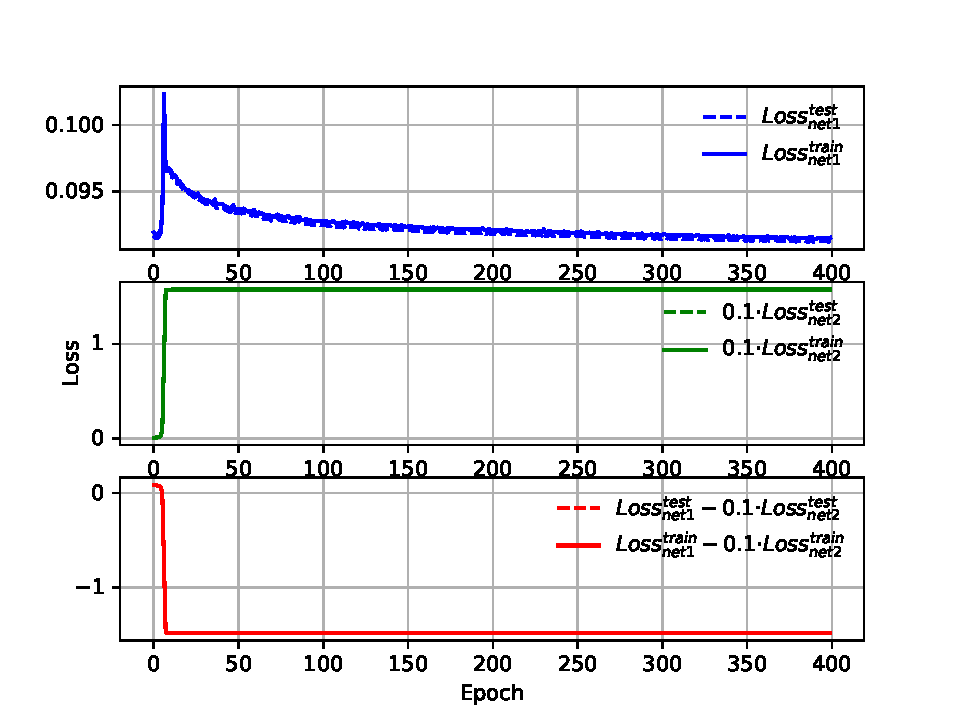
\includegraphics[width=\textwidth]{app3/app3_losses2.pdf}
        %\caption{}
        \label{fig:simple:final:sepa}
    \end{subfigure}
\quad
    \begin{subfigure}[b]{0.47\textwidth}
        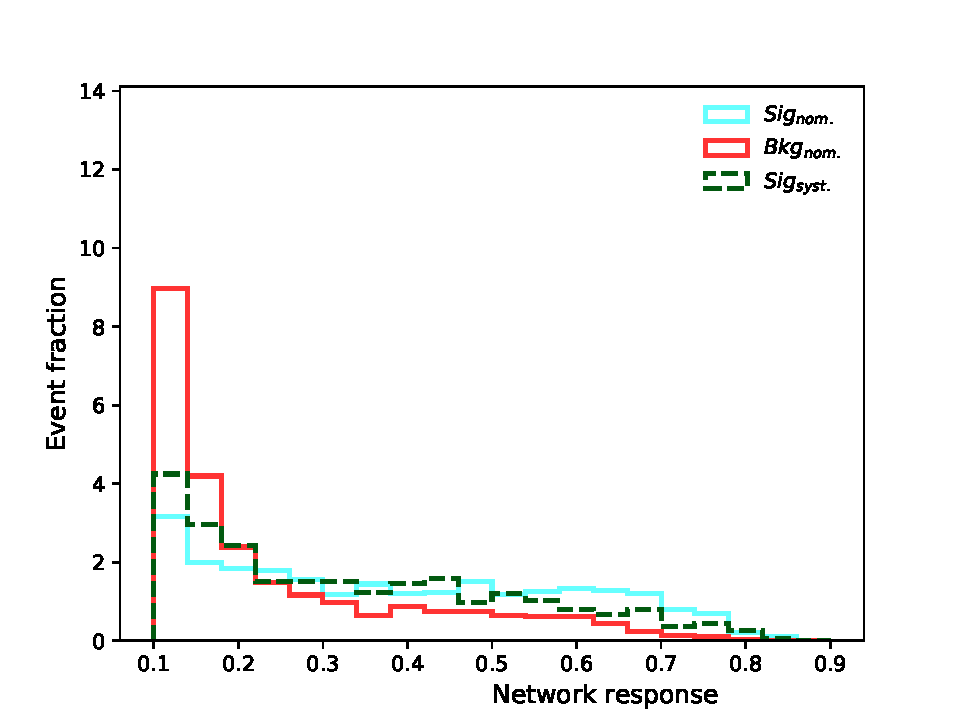
\includegraphics[width=\textwidth]{app3/app3_syst.pdf}
        %\caption{}
        \label{fig:simple:final:syst}
    \end{subfigure}
    \end{figure}
        \begin{itemize}
            \item Almost no difference
            \item Slightly higher stability
        \end{itemize}
\end{frame}


\begin{frame}{Thoughts}
    \begin{block}{Input}
        \begin{itemize}
            \item Different variable set $\rightarrow$ different problem topology
            \item Concatenate layers as input $\rightarrow$ Combination of more information and final output
            \item Separate background from the adversary's input $\rightarrow$ remove possible bias
        \end{itemize}
    \end{block}
    %
    \begin{block}{General}
        \begin{itemize}
            \item Different analysis $\rightarrow$ Insight on the network's general inability
        \end{itemize}
    \end{block}
\end{frame}

\begin{frame}{Conclusions}
    \begin{block}{Optimisation of a combination of networks}
        \begin{itemize}
            \item Classifier and adversary need to be optimised together rather than separately
        \end{itemize}
    \end{block}
    %
    \begin{block}{Input of the adversary}
        \begin{itemize}
            \item The complex architecture of the adversary is not justified by just inputting the classifier's output
        \end{itemize}
    \end{block}
    %
    \begin{block}{Strong dependency on the learning rate}
        \begin{itemize}
            \item Learning rate is the defining factor of the performance of the losses
            \item Presumably due to the fine topology around the minimum
        \end{itemize}
    \end{block}
\end{frame}

\begin{frame}{}
    \begin{figure}
        \centering
        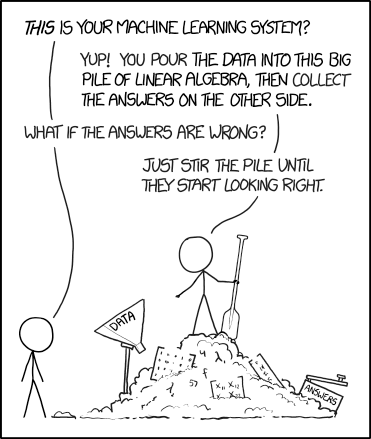
\includegraphics[width=0.4\textwidth]{xkcd}
        \caption{https://xkcd.com/1838/}
    \end{figure}
\end{frame}


%\begin{frame}{Sources}

%\printbibliography
    
%\end{frame}





\begin{frame}{Neural Networks}
\begin{columns}
    \begin{column}{0.5\textwidth}
    \begin{itemize}
        \item Built of layers of simple processors called nodes
        \item Each node is connected to each node in the surrounding layers
        \item The connection is built by a linear function with a weight $\omega$ and a bias $b$ 
        and a non linear activation function $\sigma$
        \item Learning is accomplished by backpropagation and a step optimizer
    \end{itemize}
    \end{column}
    \begin{column}{0.5\textwidth}
    \begin{figure}
        \centering
        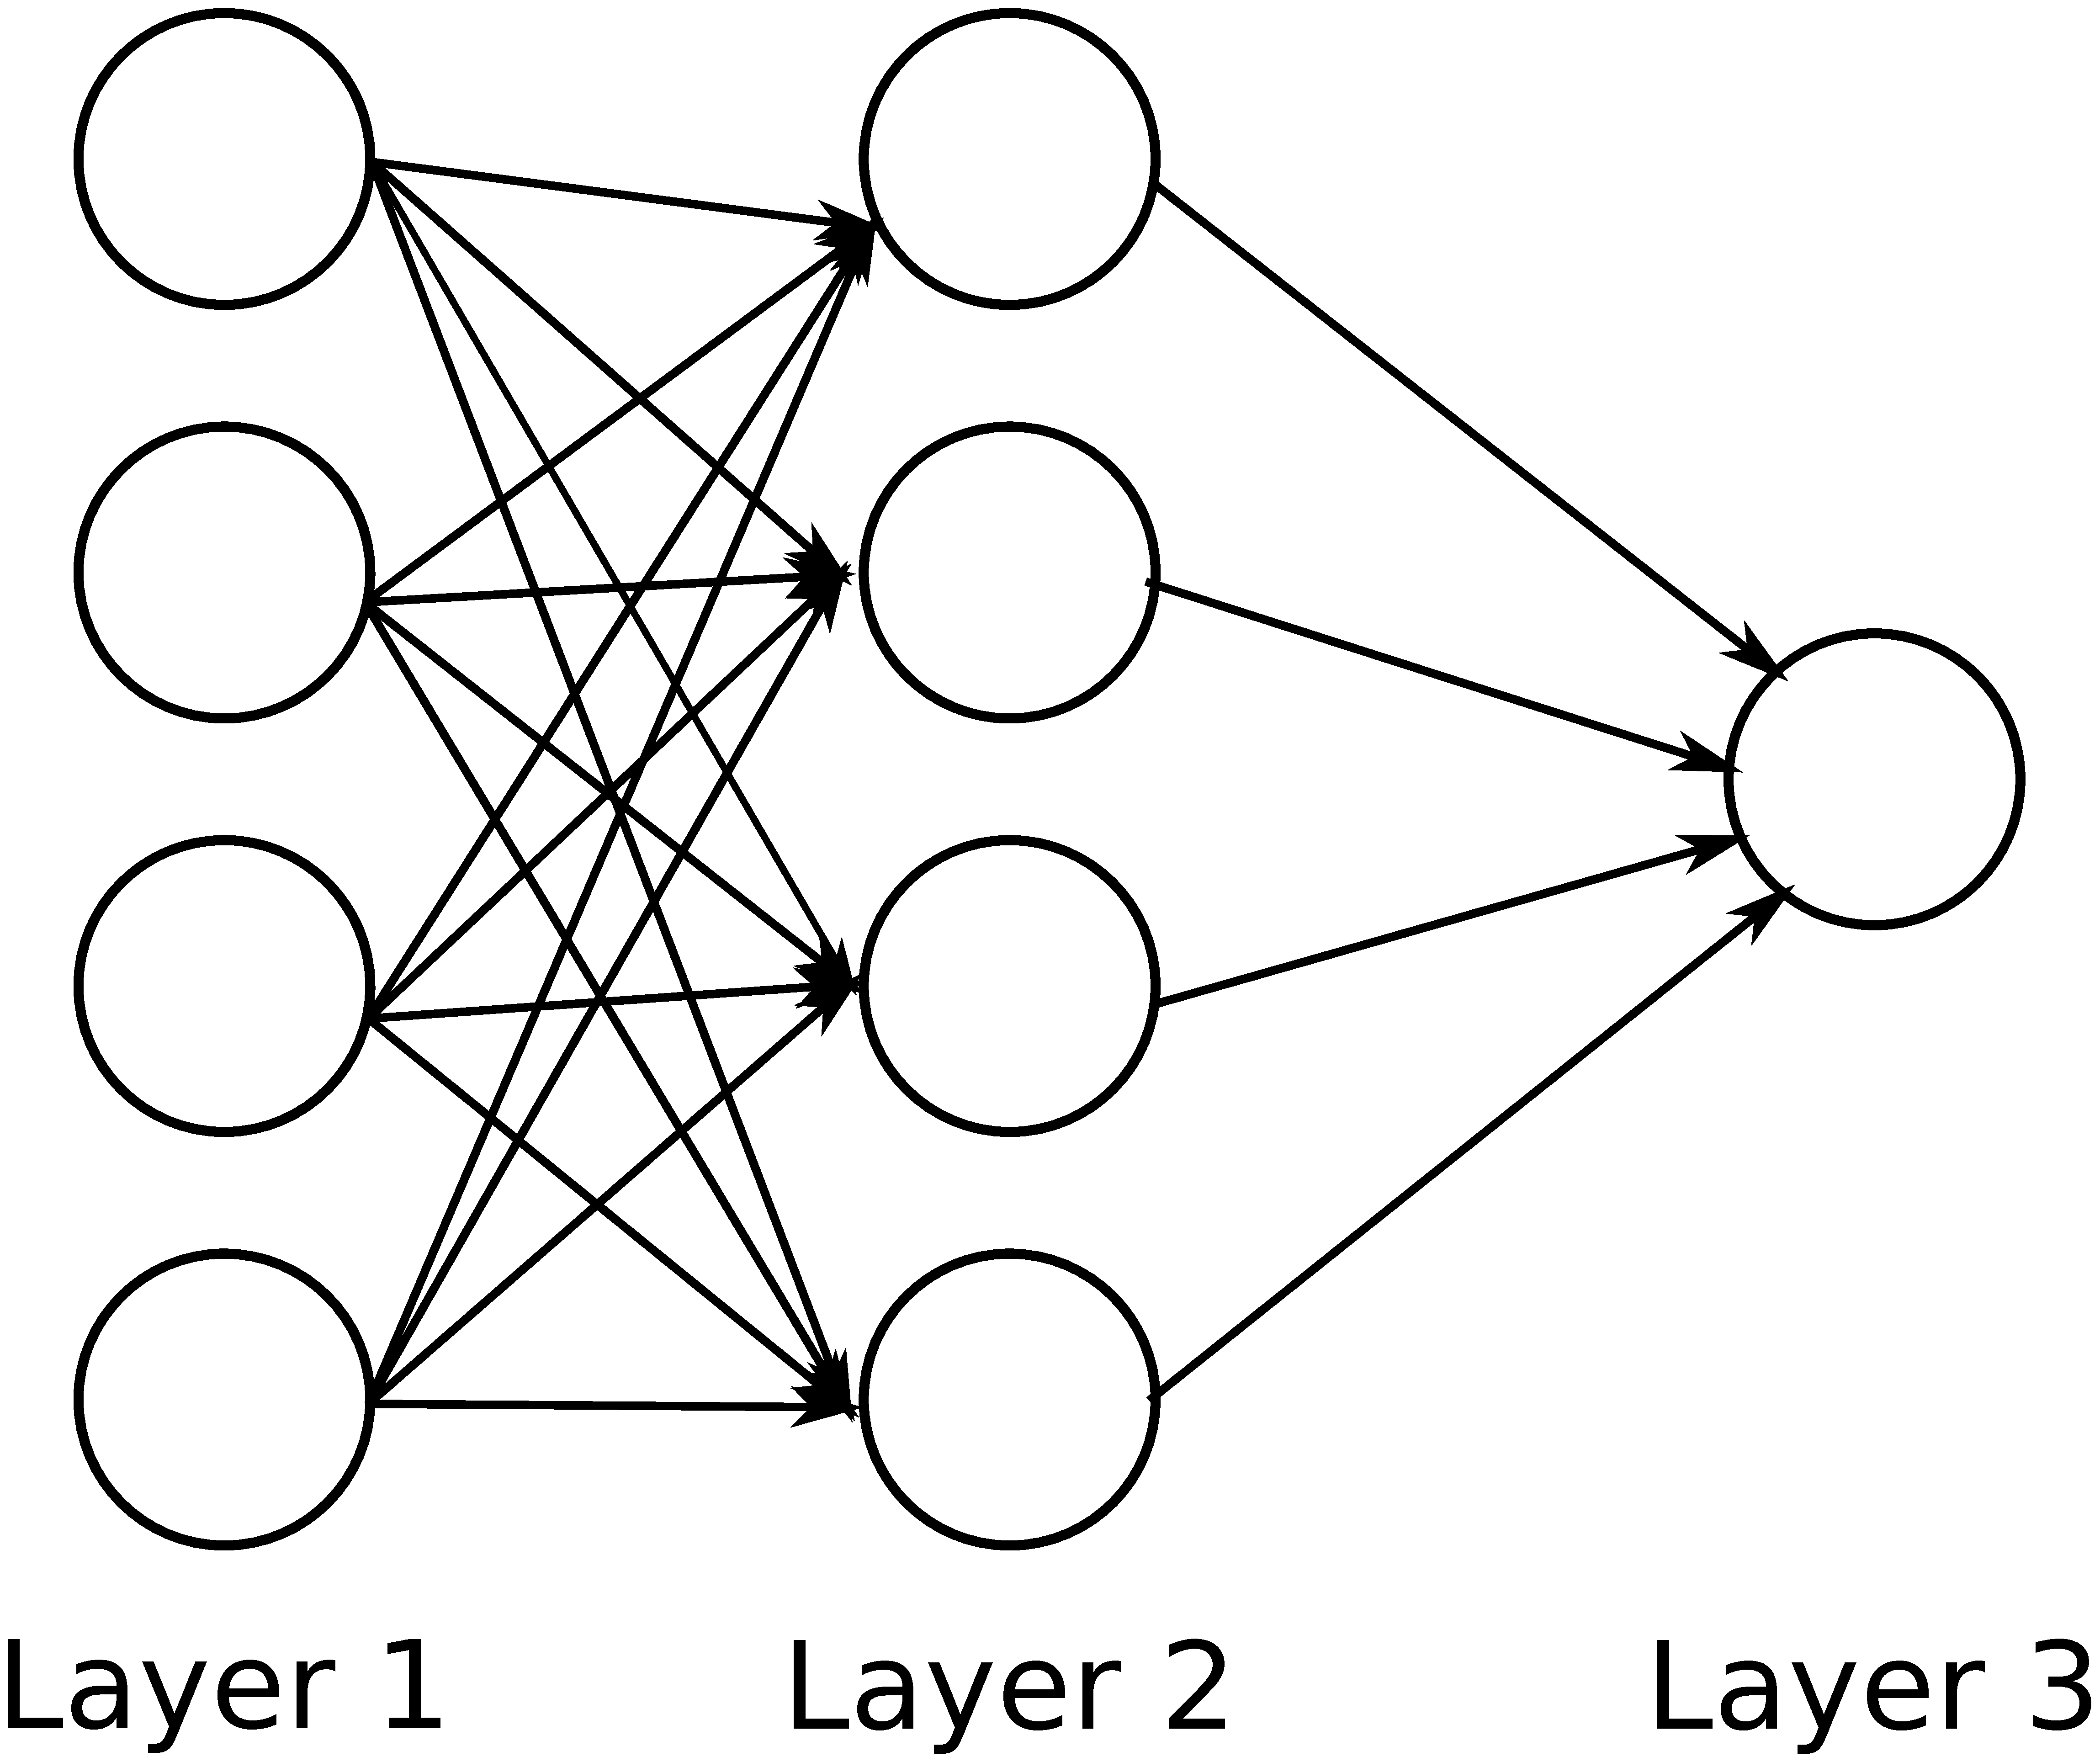
\includegraphics[scale=0.05]{network.eps}
        \label{fig:my_label}
    \end{figure}
    \vspace{0.3cm}
    \begin{center}
     $z_j^L = \omega_{jk}^L a_k^{L-1} + b_k$\\
        $a_j^L = \sigma ( z_j^L )$
    \end{center}
    \end{column}
\end{columns}
\end{frame}

\begin{frame}{Neural Networks}
\begin{figure}
    \centering
    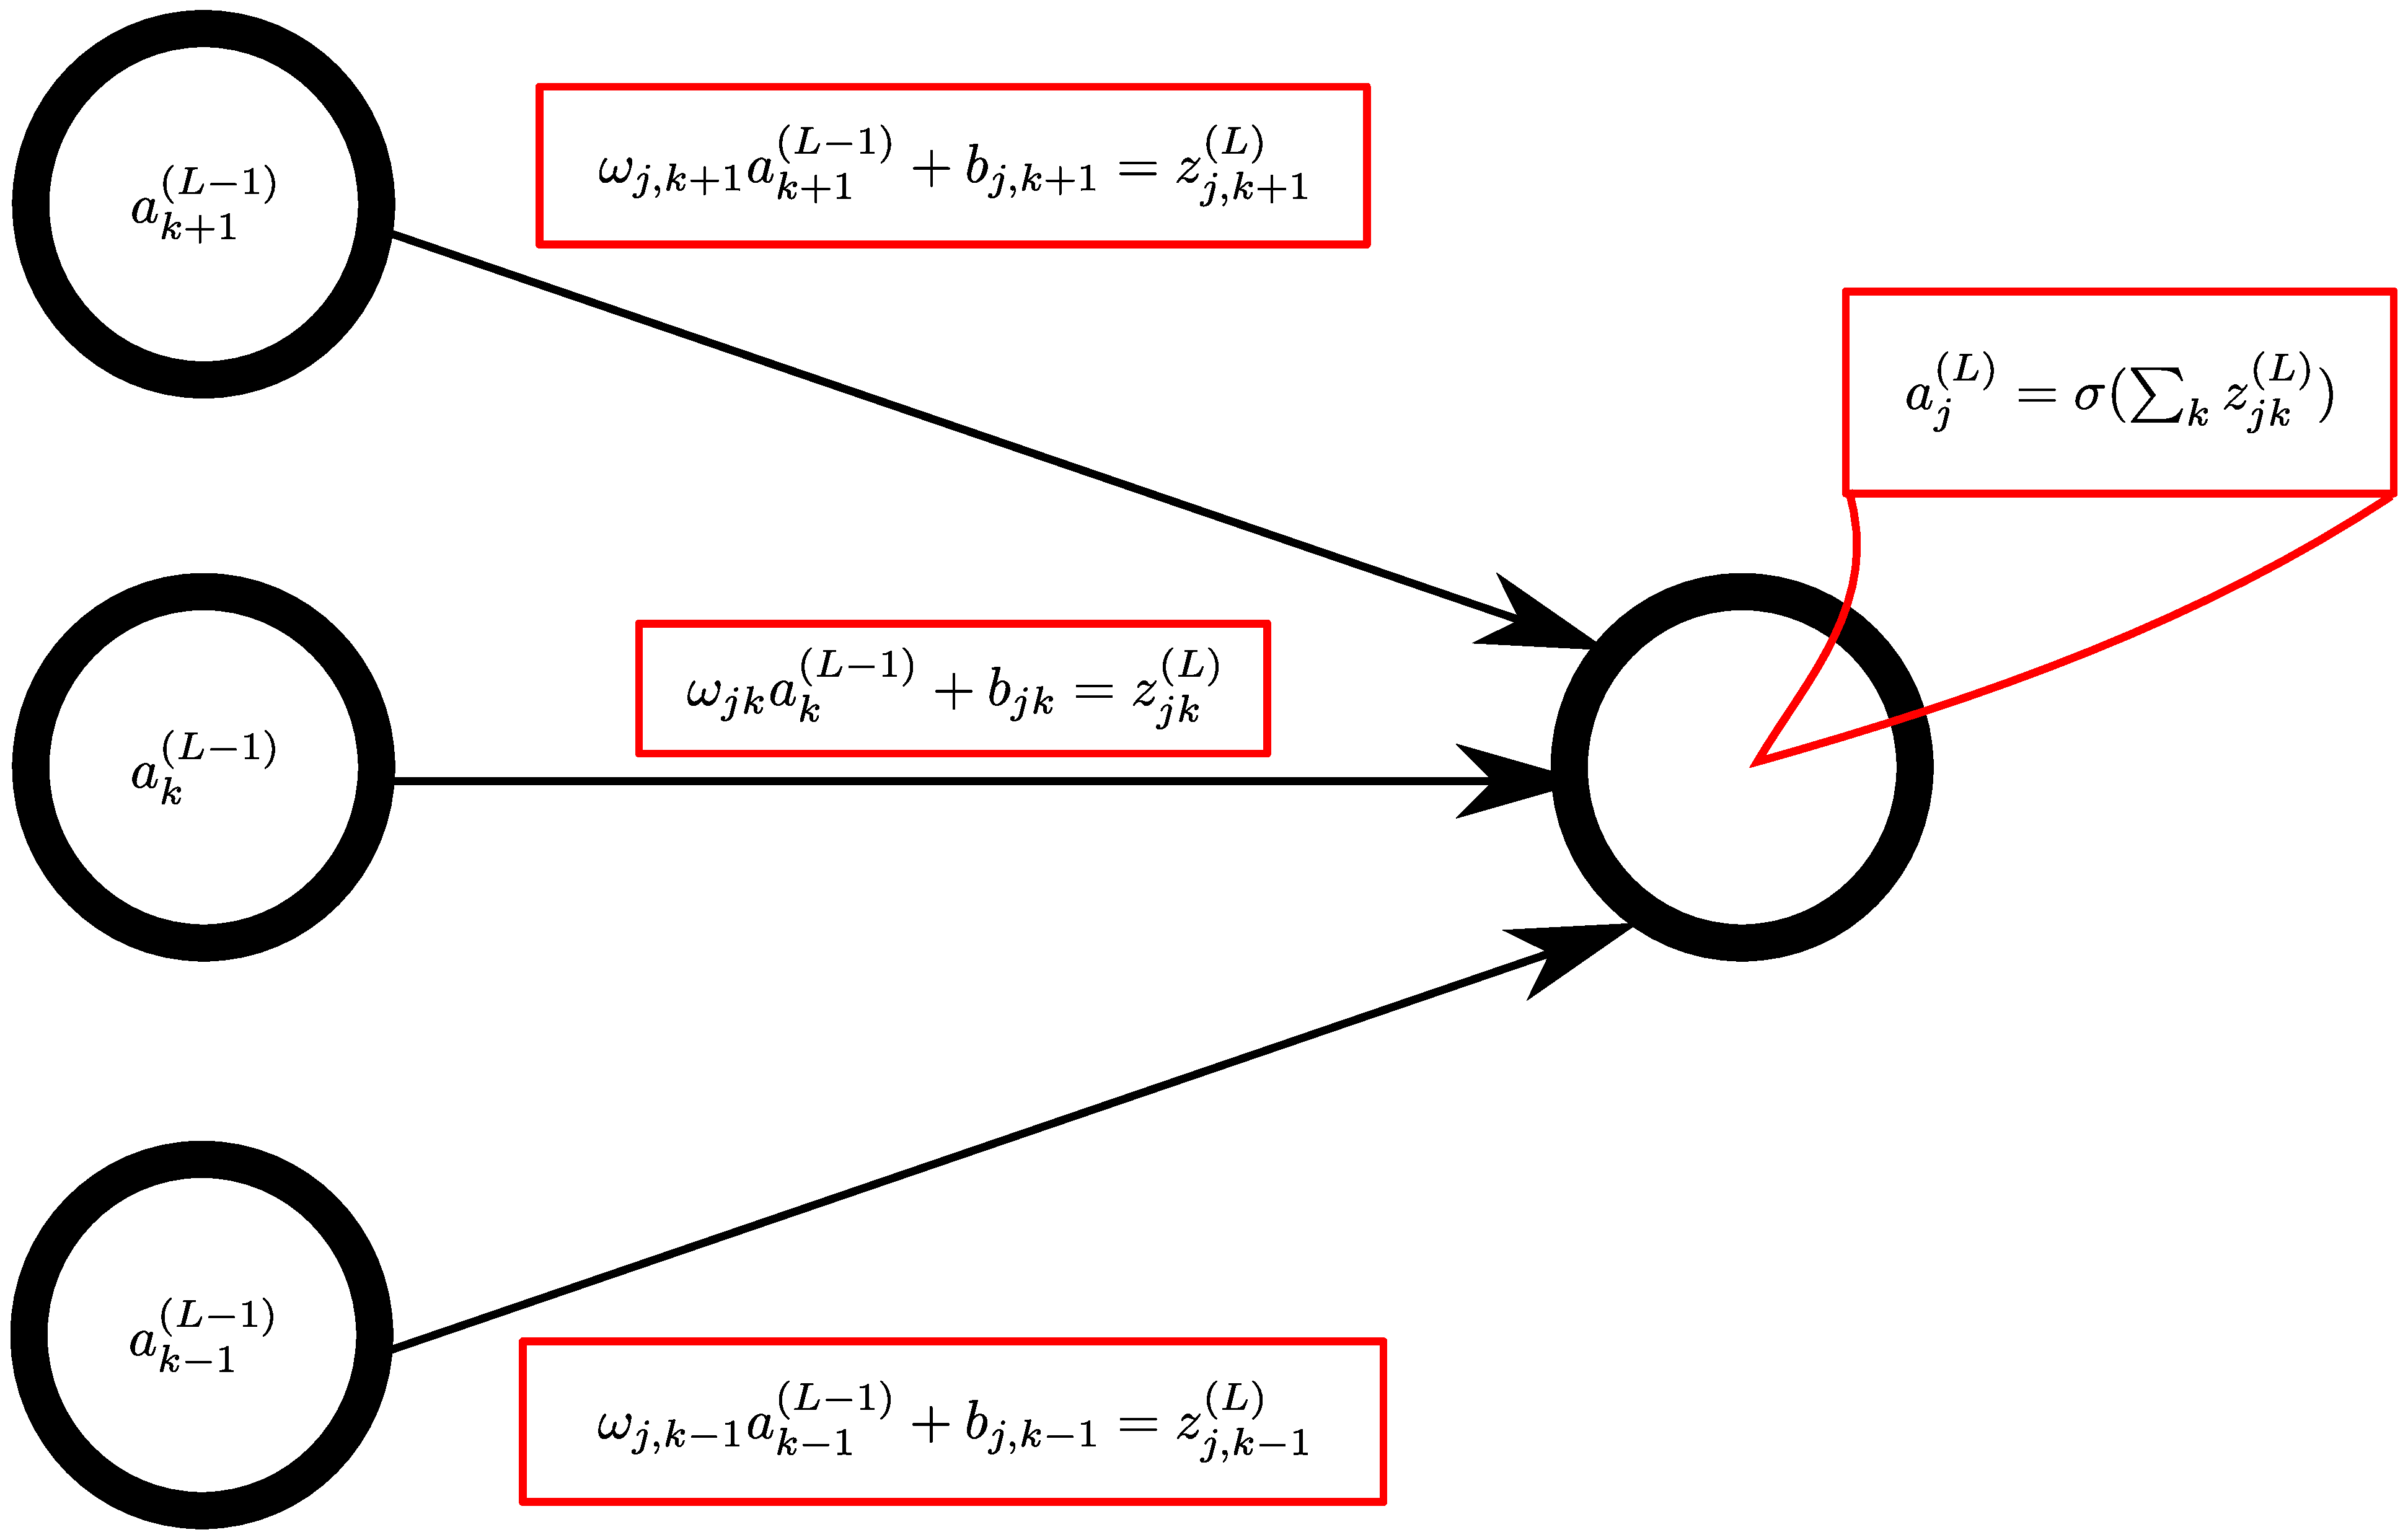
\includegraphics[scale=0.15]{nodes_nomenclature.eps}
    \caption{Forward Propagation in a neural network}
    \label{fig:my_label}
\end{figure}
\end{frame}

\begin{frame}{Choosing the next step}
    \begin{itemize}
        \item In supervised learning truth tagged training data allows to calculate a cost function to estimate a model's quality. For example crossentropy:
        \begin{align}
            C = -(y \log p + (1 - y) \log (1 - p) )
            \label{eq:binary_crossentropy}
        \end{align}
        \item Backpropagation estimates the parameters' impact on the cost function using the partial derivatives
        \begin{align*}
            \frac{\partial C}{\partial a_k^{L-1}} = \sum_{j=1}^N \frac{\partial z_j^L}{\partial a_k^{L-1}} \frac{\partial a_j^L}{\partial z_j^L}\frac{\partial C}{\partial a_j^L}
        \end{align*}
        \item Each parameter is then updated accoring to its impact on the cost function
    \end{itemize}
\end{frame}


\begin{frame}{Adversarial Neural Networks}
    \begin{itemize}
        \item Originally introduced as Generative adversarial neural networks to overcome weaknesses of generative networks \cite{2014arXiv1406.2661G}
        \item Adds a second network controlling the dependency on features with large systematic uncertainties. 
        \item The adversarial structure of the networks creates a minimax game
        \item Combined loss function
    \end{itemize}
\end{frame}

\begin{frame}{Optimisers}
\begin{itemize}
    \item Gradient Descent: Update parameters in the opposite direction of the error gradient
    \item Stochastic Gradient Descent: Gradient Descent but for each training example separately
    \item Adaptive Moment Estimation, Adam: adaptive learning rate based on exponentially decaying mean of past gradients and past square gradients.
    \item Others
    \item https://towardsdatascience.com/types-of-optimization-algorithms-used-in-neural-networks-and-ways-to-optimize-gradient-95ae5d39529f
\end{itemize}
    
\end{frame}



\begin{frame}{Learning rate, momentum, decay}
\begin{itemize}
    \item Learning rate: Step-length in gradient direction
    \begin{align}
    \theta^{\prime} = \theta - lr \cdot g
    \end{align}
    \item Momentum: create an adaptive and weight dependent learning rate
    \begin{align}
    \nu^{\prime} = \alpha \nu - \epsilon \frac{1}{m} \nabla_{\theta} \sum_j L(f(\hat{y}^j; \theta), y^j)\\
    \theta^{\prime} = \theta + \nu
    \end{align}
    \item Decay: Decrease the learning rate over the course of the training
    \begin{align}
    \epsilon^{\prime} = \frac{\epsilon}{1 + \phi t}
    \end{align}
\end{itemize}
\end{frame}


\begin{frame}{Dropout}
\begin{figure}
    \centering
    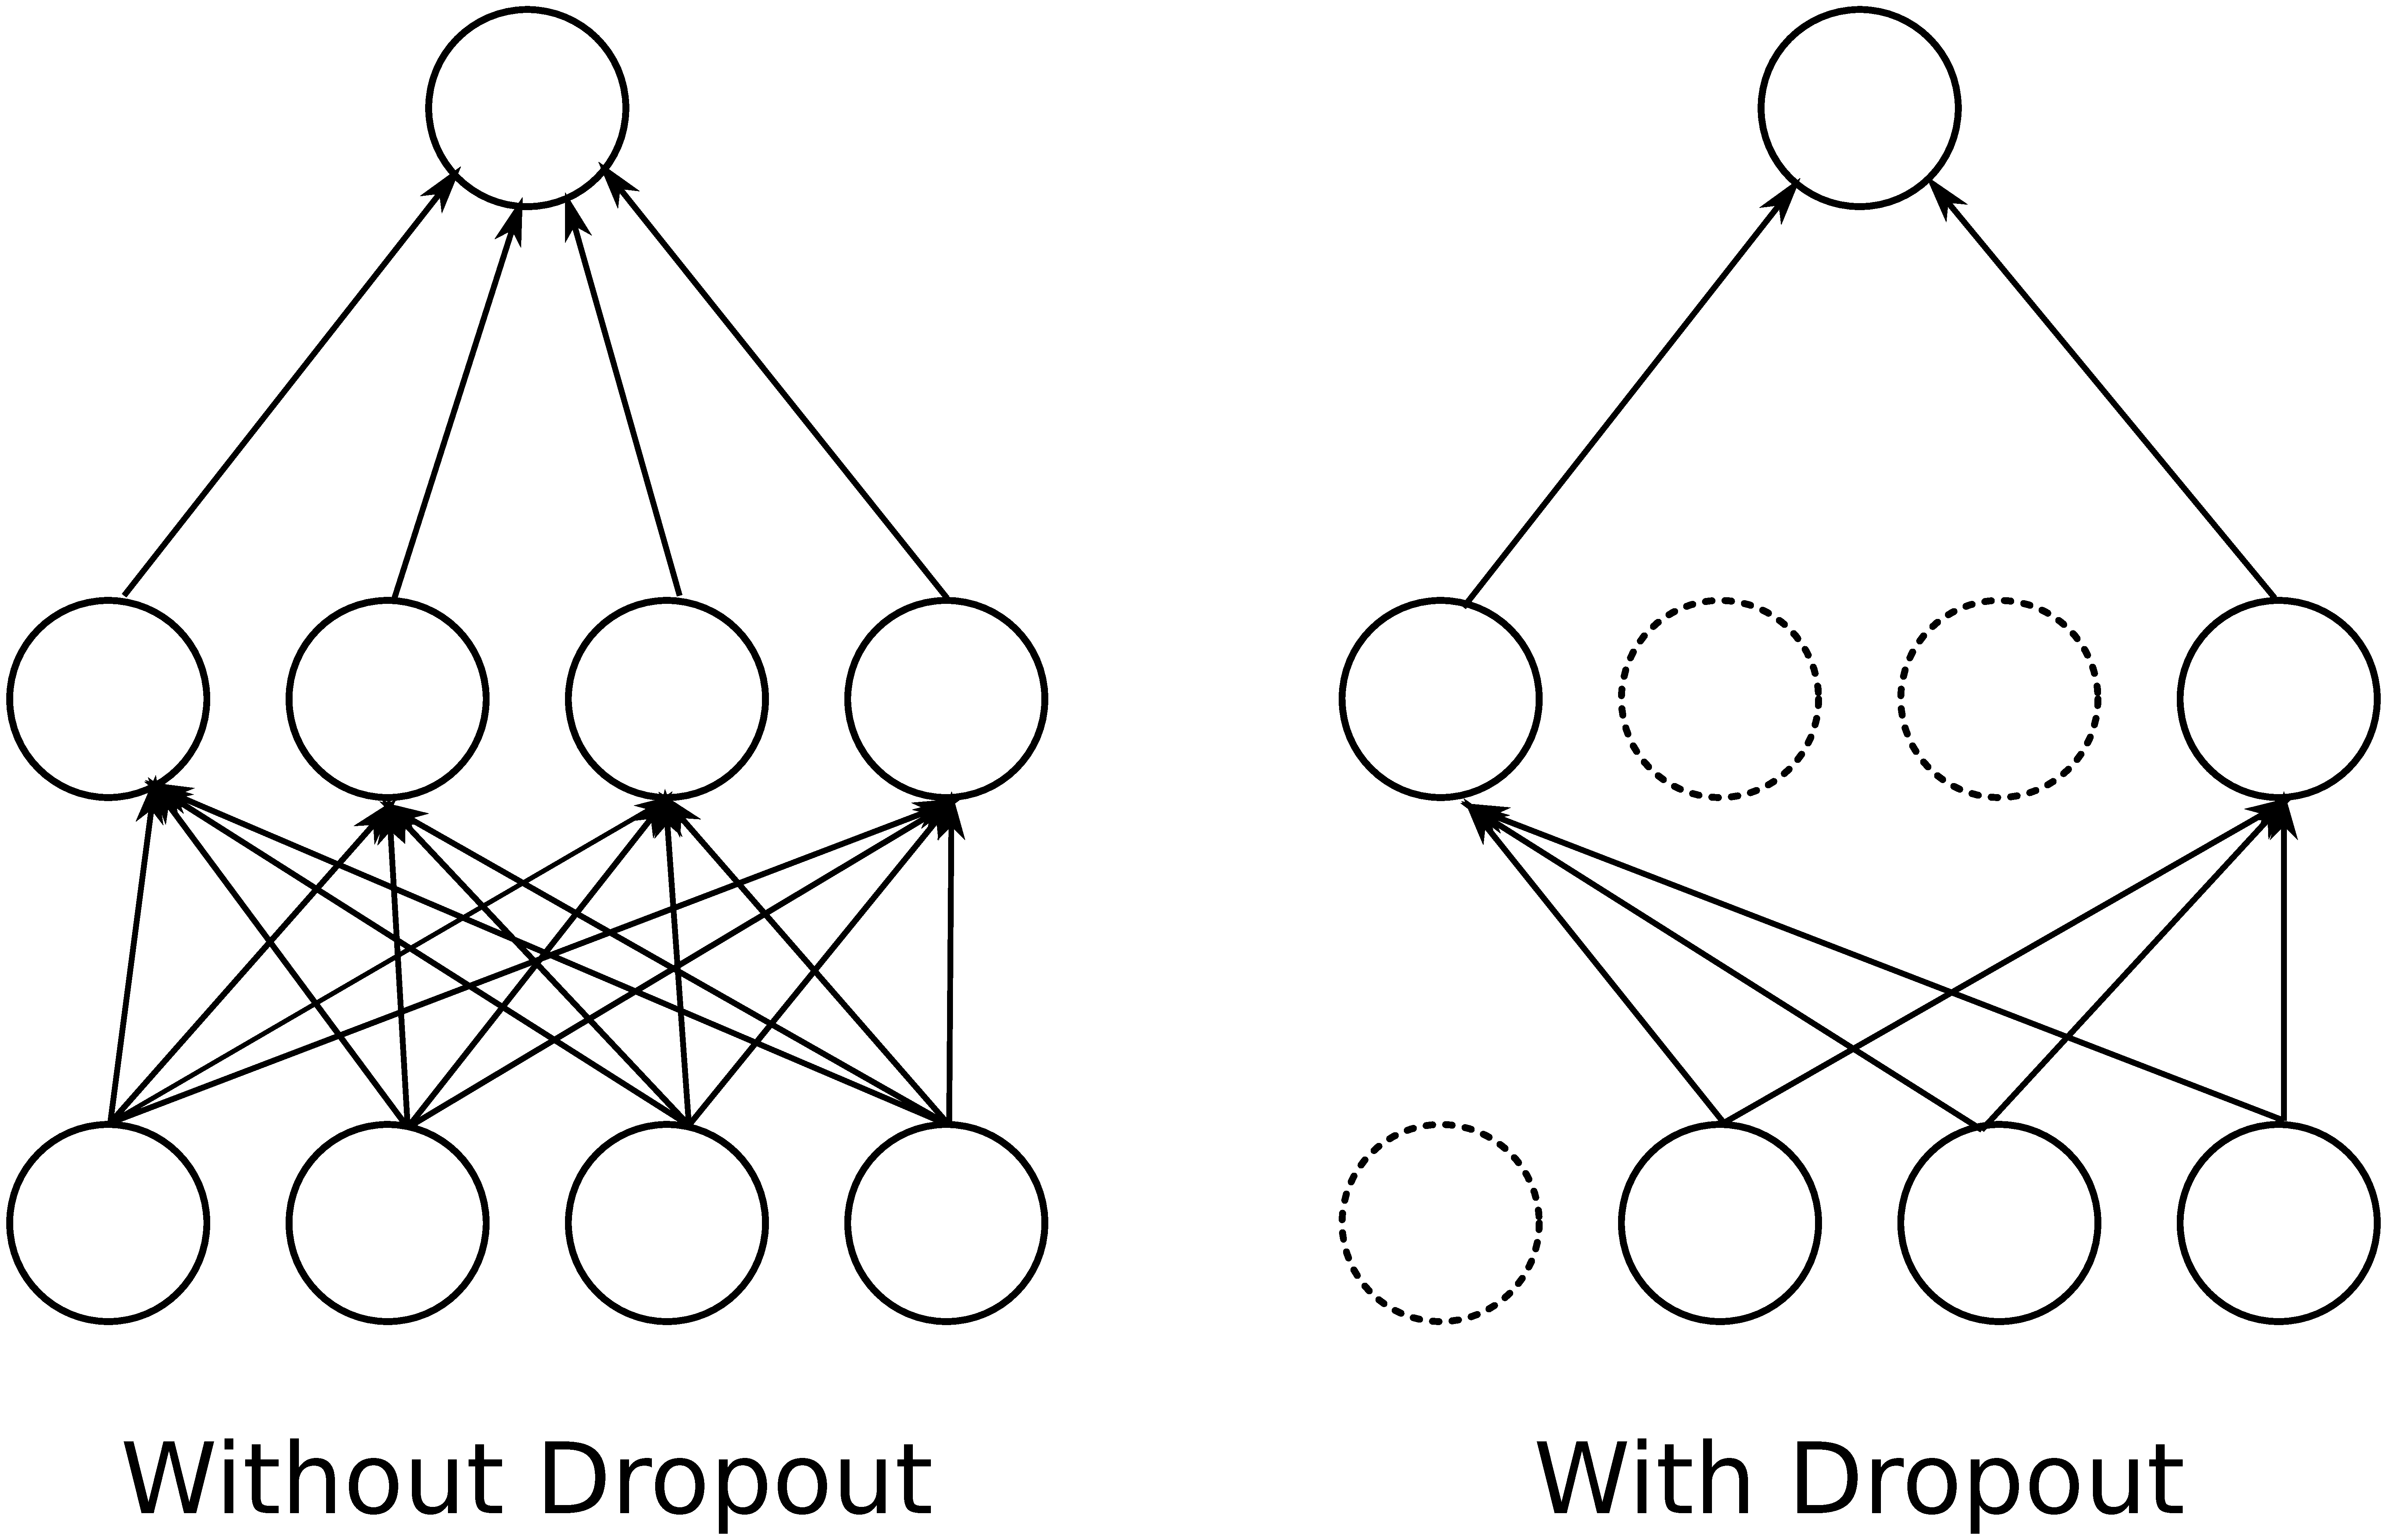
\includegraphics[scale=0.07]{dropout.eps}
    \caption{Caption}
    \label{fig:my_label}
\end{figure}
\end{frame}

\begin{frame}{Technical details}
    \begin{itemize}
        \item The neural networks were built using Keras \cite{chollet2015keras} with tensorflow \cite{tensorflow2015-whitepaper} as backend
    \end{itemize}
\end{frame}

\begin{frame}{Variables}
Inhalt...
\end{frame}




\end{document}